\documentclass[a4paper,11pt]{book}
\usepackage{lmodern}
\usepackage{circuitikz}
\usepackage{amssymb,amsmath}
\usepackage{siunitx}
\usepackage{ulem}

% use upquote if available, for straight quotes in verbatim environments
\IfFileExists{upquote.sty}{\usepackage{upquote}}{}

% use microtype if available
\IfFileExists{microtype.sty}{%
\usepackage[]{microtype}
\UseMicrotypeSet[protrusion]{basicmath} % disable protrusion for tt fonts
}{}

% This requires pdflatex -shell-escape
\usepackage{minted}

\usepackage[colorinlistoftodos]{todonotes}
\newcommand{\mtodo}{\todo[inline]}

\PassOptionsToPackage{hyphens}{url} % url is loaded by hyperref
\usepackage[unicode=true]{hyperref}
\hypersetup{pdfborder={0 0 0},
  breaklinks=true}

\hypersetup{colorlinks=true, linkcolor=blue, urlcolor=blue, citecolor=green}

\urlstyle{same}  % don't use monospace font for urls
\usepackage{graphicx,grffile}
\makeatletter
\def\maxwidth{\ifdim\Gin@nat@width>\linewidth\linewidth\else\Gin@nat@width\fi}
\def\maxheight{\ifdim\Gin@nat@height>\textheight\textheight\else\Gin@nat@height\fi}
\makeatother

% Scale images if necessary, so that they will not overflow the page
% margins by default, and it is still possible to overwrite the defaults
% using explicit options in \includegraphics[width, height, ...]{}
\setkeys{Gin}{width=\maxwidth,height=\maxheight,keepaspectratio}
\IfFileExists{parskip.sty}{%
\usepackage{parskip}
}{% else
\setlength{\parindent}{0pt}
\setlength{\parskip}{6pt plus 2pt minus 1pt}
}

\setlength{\oddsidemargin}{0mm}
\setlength{\evensidemargin}{-14mm}
\setlength{\marginparwidth}{0cm}
\setlength{\marginparsep}{0cm}
\setlength{\topmargin}{2mm}
\setlength{\textwidth}{168mm}
\setlength{\textheight}{240mm}
\setlength{\footskip}{10mm}

\setlength{\emergencystretch}{3em}  % prevent overfull lines
\providecommand{\tightlist}{%
  \setlength{\itemsep}{0pt}\setlength{\parskip}{0pt}}

%\setcounter{secnumdepth}{0}

% Redefines (sub)paragraphs to behave more like sections
\ifx\paragraph\undefined\else
\let\oldparagraph\paragraph
\renewcommand{\paragraph}[1]{\oldparagraph{#1}\mbox{}}
\fi
\ifx\subparagraph\undefined\else
\let\oldsubparagraph\subparagraph
\renewcommand{\subparagraph}[1]{\oldsubparagraph{#1}\mbox{}}
\fi

% set default figure placement to htbp
\makeatletter
\def\fps@figure{htbp}
\makeatother

\newcommand{\program}[1]{\texttt{#1}}
\newcommand{\code}[1]{\mintinline{C}{#1}}
\newcommand{\file}[1]{\texttt{#1}}
\newcommand{\wfile}[1]{\href{https://eng-git.canterbury.ac.nz/wacky-racers/wacky-racers/-/blob/master/src/#1}{\mintinline{bash}{wacky-racers/src/#1}}}
\newcommand{\wikiref}[2]{\href{http://ecewiki.elec.canterbury.ac.nz/mediawiki/index.php/#1}{\mintinline{bash}{#2}}}
\newcommand{\pin}[1]{\texttt{#1}}
\newcommand{\sig}[1]{\texttt{#1}}
\newcommand{\ud}{\mathrm{d}}                    % upright d (derivative)

\newcommand{\reffig}[1]{\mbox{Figure~\ref{fig:#1}}}
\newcommand{\reftab}[1]{\mbox{Table~\ref{tab:#1}}}
\newcommand{\refeqn}[1]{\mbox{(\ref{eqn:#1})}}

\title{The Wacky Racers Guide, V1.010}
\author{Michael Hayes and Mutley}
\date{\today\\[2cm] 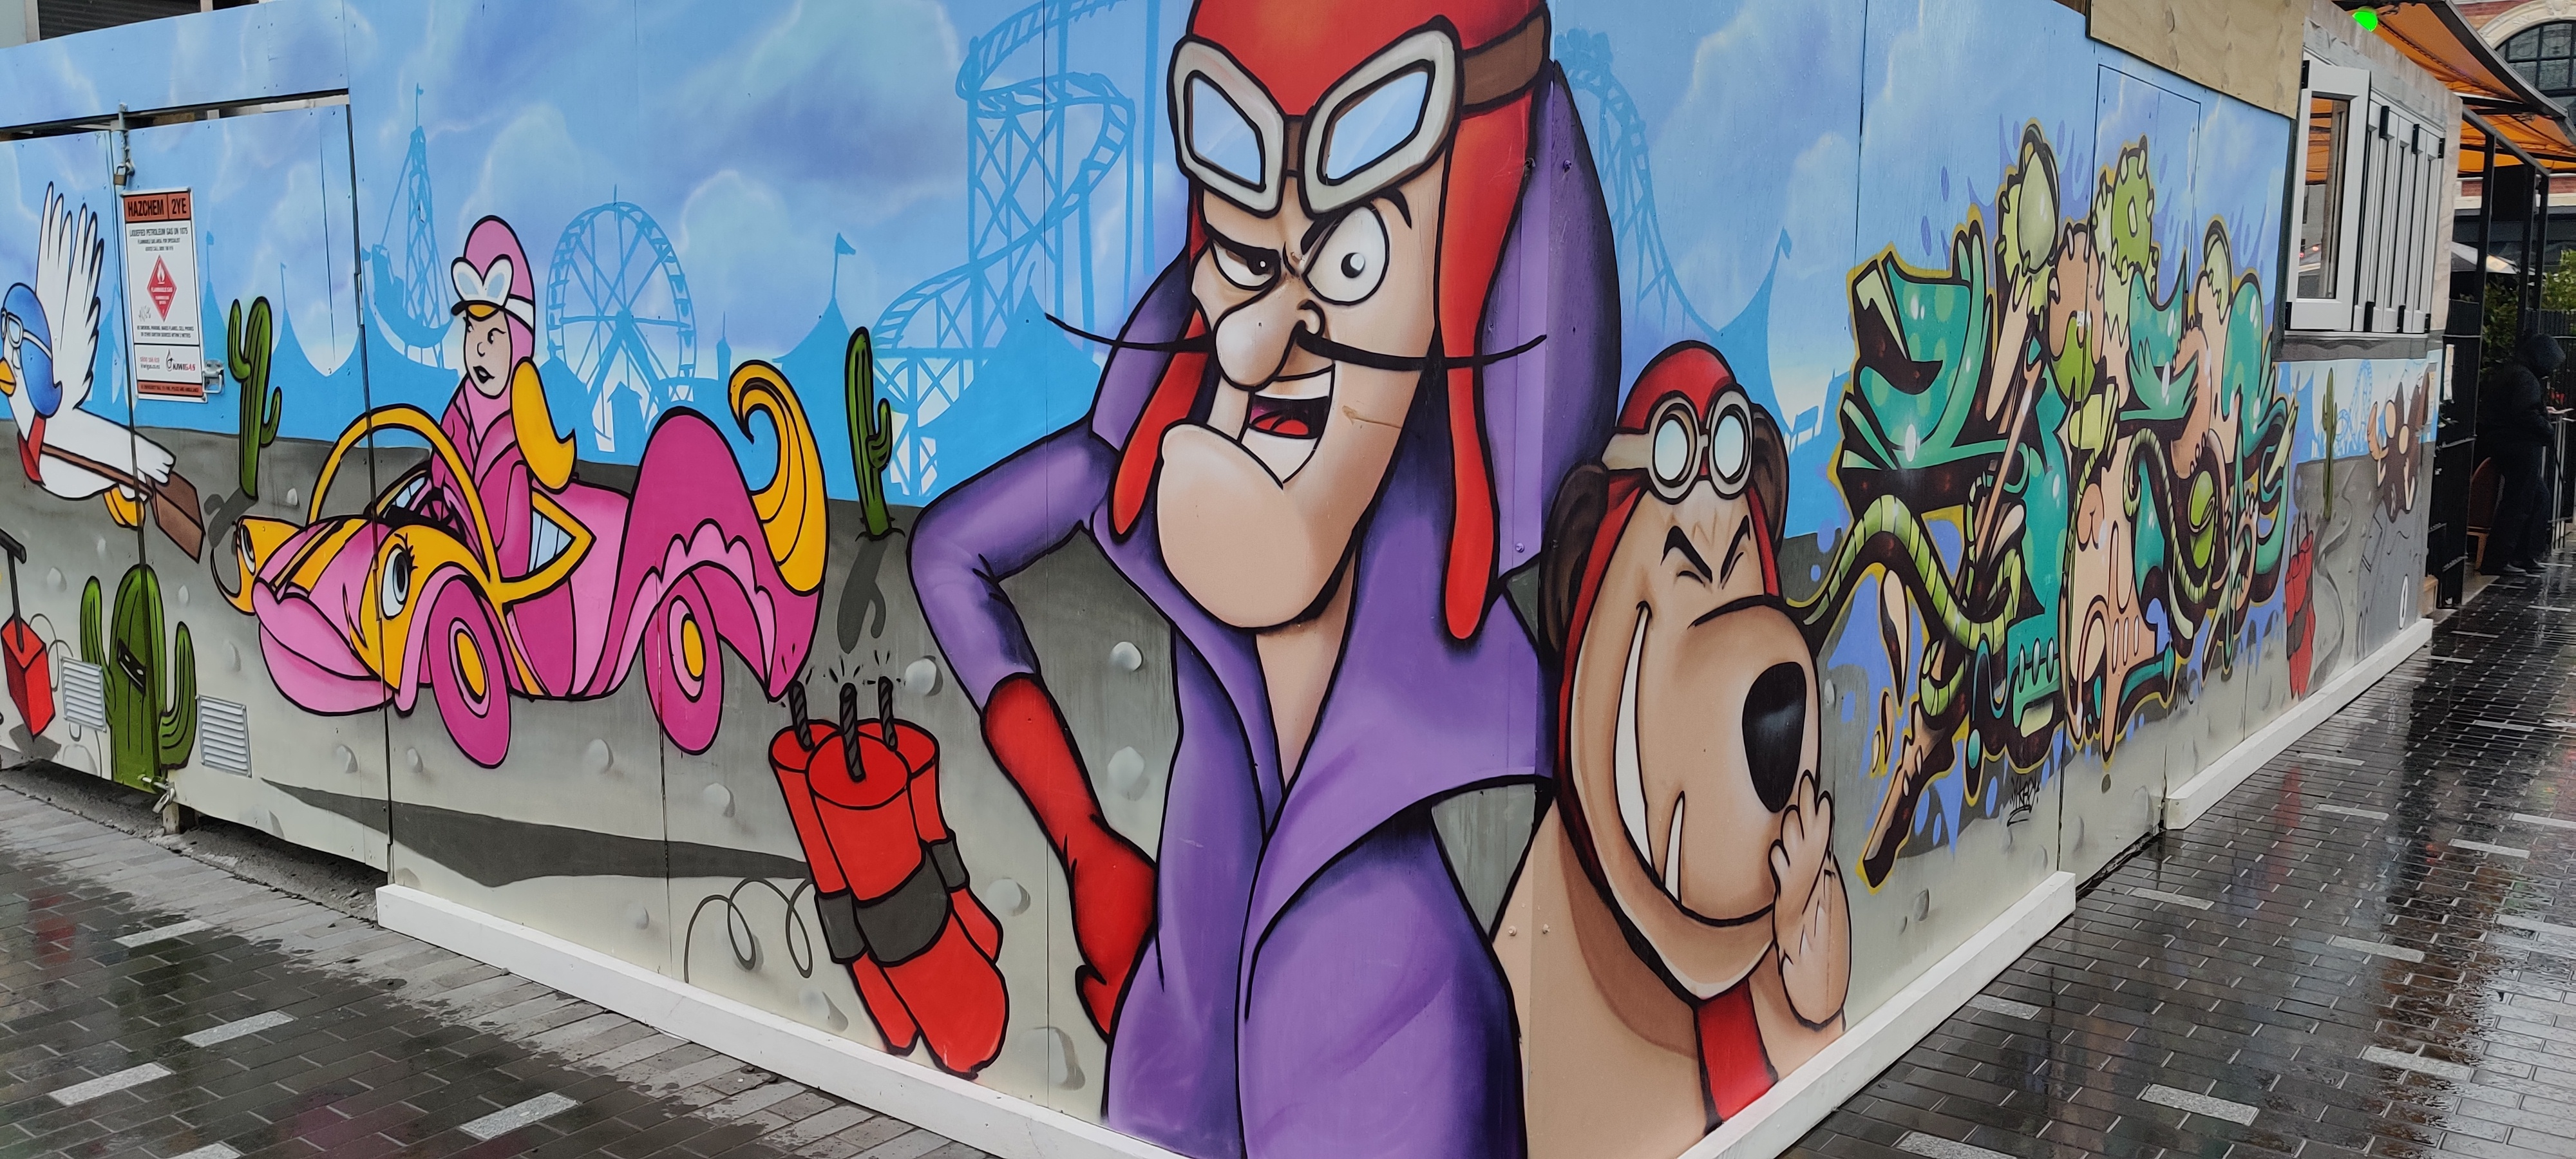
\includegraphics{figs/wacky_mural.jpg}}

\begin{document}
\maketitle

\tableofcontents

%\chapter{Requirements}




%\chapter{Schedule}

\begin{description}
\item [Term~1 week~1]\mbox{}\\

  \begin{itemize}
  \item Form a group of four and register your group on Learn.
  %\item Read the \hyperref[requirements]{requirements section}.
  \item Read the requirements section in the instructions document.
  \item Peruse the datasheets of the key components.
  \end{itemize}
  
\item [Term~1 week~2]\mbox{}\\
  
  \begin{itemize}
  \item Attend Altium schematic tutorial.
  \item Start your schematic design.
  \item Read suggestions in \hyperref[hardware]{hardware section}.
  \end{itemize}
  
\item [Term~1 week~3]\mbox{}\\
  
  \begin{itemize}
  \item Submit you Altium schematic for review.
  \item Attend review feedback session.
  \end{itemize}
  
\item [Term~1 week~4]\mbox{}\\
  
  \begin{itemize}
  \item Attend Altium PCB tutorial.
  \item Start your PCB layout.
  \end{itemize}
  
  
\item [Term~1 week~5]\mbox{}\\
  
  \begin{itemize}
  \item Attend SMT lab induction.
  \item Submit PCB design (early round).
  \end{itemize}
  
  
\item [Term~1 week~6]\mbox{}\\  
  
  \begin{itemize}
  \item Submit PCB design (late round).
  \end{itemize}
  
  
\item [Break week~1]\mbox{}\\
  
  
\item [Break week~2]\mbox{}\\  
  
  \begin{itemize}
  \item Populate and test PCB.
  \end{itemize}
  
  
\item [Break week~3]\mbox{}\\
  
  \begin{itemize}
  \item Populate and test PCB.
  \end{itemize}  
  
  
\item [Term~2 week~1]\mbox{}\\
  
  \begin{itemize}
  \item Demonstrate blinky program.
  \end{itemize}
  
  
\item [Term~2 week~2]\mbox{}\\
  
  \begin{itemize}
  \item Demonstrate IMU/motors functionality.
  \end{itemize}
  
  
\item [Term~2 week~3]\mbox{}\\
  
  \begin{itemize}
  \item Demonstrate IMU/motors functionality.
  \end{itemize}
  
\item [Term~2 week~4]\mbox{}\\  
  
  \begin{itemize}
  \item Demonstrate radio control.
  \end{itemize}  
  
\item [Term~2 week~5]\mbox{}\\
  
  \begin{itemize}
  \item Demonstrate full functionality.
  \item Plan your costumes!
  \end{itemize}
  
\item [Term~2 week~25]\mbox{}\\
  
  \begin{itemize}
  \item Practice control of you wacky racer.
  \item Attend wacky race.
  \item Submit PCB for inspection (box in SMT lab).
  \item Return chassis and batteries.
  \item Submit individual critique to Learn.    
  \end{itemize}
  
\end{description}

\chapter{Introduction}

This guide is written in the hope that it will ease your introduction
into building, programming, and troubleshooting an embedded system.
Making embedded systems is not easy; you have to get a lot right.  One
incorrect bit can be the difference between a working and a
non-working system.

If you find things a little Linux-centric, well that's the only
operating system I've run for over twenty-five years.  It is a common
operating system for many high-end embedded systems; it runs on
Android phones and probably on your internet router.  And, yeah, I
like the command-line; it is faster than using a mouse and GUI.


\label{hardware}
\chapter{Hardware}



\section{Recommendations}\label{recommendations}

\begin{enumerate}
\item
  Independently fuse the buck converter and H-bridge. This allows a fuse
  to be removed to isolate part of the circuit when finding a fault,
  such as a short across the power rails.

\item
  Have a zener diode to protect against overvoltage when your group
  member inadvertently cranks up the voltage from the bench power
  supply.

\item
  Have current limiting resistors for all off-board signals.

\item
  Have plenty of testpoints, especially for power supplies and
  signals.  You will never have enough!

\item
  Have at least one grunty ground testpoint for attaching a scope ground
  clip.

\item
  Have a dedicated PIO pin to drive a testpoint that you can use to
  trigger an oscilloscope for debugging.

\item
  Have the SAM4S erase pin connected to a test point close to a 3.3\,V
  testpoint. This is useful to completely erase the SAM4S flash memory
  when nothing works.

\item
  Have a MOSFET or servo interface for controlling something dastardly!
  
\end{enumerate}

\section{SAM4S MCU}\label{sam4s-mcu}

The SAM4S MCU is overkill for this assignment but is typical of
ARM processors used for bare-metal applications.

\subsection{Power pins}\label{power-pins}

The SAM4S has four grounds. They \textbf{must} all be connected. There
are also seven power pins. These \textbf{must} all be connected since
they power different parts of the chip. Note, some pins require 3.3\,V
while others require 1.2\,V. The 1.2\,V is generated by an internal
voltage regulator.

\subsection{Peripheral pins}\label{peripheral-pins}

\textbf{Many of the peripheral pins are dedicated and cannot be
reassigned in software}, e.g., SPI, TWI, and USB pins. Note, there are
restrictions on the PWM pins.

By default the \pin{PB4} and \pin{PB5} pins are configured for the JTAG debugger.
These can be used for general PIO after setting an internal bit.  See
\protect\hyperref[disabling-jtag-pins]{disabling JTAG pins}.

The logic levels are set by the voltage on the VDDIO pin (usually
3.3\,V).  \pin{PA12}--\pin{PA14} and \pin{PA26}--\pin{PA31} can sink/source
4\,mA.  The USB pins (\pin{PB10}--\pin{PB11}) can sink/source 30\,mA.  The
rest can only sink/source 2\,mA of current.


\subsection{USART/UART}\label{usartuart}

The SAM4S has two USARTs and two UARTs. The USARTs can emulate a
UART, have hardware flow control, and have a better driver so they are
recommended if you need a UART interface.


\subsection{PWM}\label{pwm}

The SAM4S can generate four independent PWM signals. There are
restrictions on which SAM4S pins they come out on. Note, the PWMLx and
PWMHx signals are complementary (i.e., one is low while the other is
high).

\subsection{TWI}\label{twi}

The SAM4S has two TWI peripherals (that can act as a master and
a slave) with dedicated TWD and TWCK pins. External pull-up resistors
are required.  TWI1 shares pins with JTAG; you will need to disable
JTAG in software.

\subsection{SPI}\label{spi}

The SAM4S has a single SPI peripheral with dedicated SCK, MISO, and
MOSI pins. Any PIO pin can be used for the chip select\footnote{For
  high speed operation (not needed for this assignment), you should
  use one of the dedicated chip select pins.}.

\subsection{ADC}\label{adc}

The SAM4S has a single ADC with a multiplexer to select one of a
number of analogue inputs.  It can sample at 1\,MHz.

\subsection{USB}\label{usb}

The SAM4S has a single USB peripheral connected to the DDP and DDM
pins. 27 ohm series termination resistors are required, placed close to
the SAM4S.

\section{Other chips}\label{other-chips}

\subsection{DRV8833 dual H-bridge}\label{drv8833-dual-h-bridge}

The H-bridge has four modes: forward, reverse, slow decay (brake), and
fast decay (coast).  With slow decay mode, the motor is shorted so
that it stops faster.  With fast decay mode, the motor is
open-circuited and so it takes longer to stop.  However, there is
little difference in practice, due to friction in the gearbox.

If you want control over fast decay and slow decay in both forward and
reverse you will need \textbf{four} independent PWM signals. The SAM4S
can provide four independent PWM signals but be \textbf{careful} since
PWMxH and PWMxL are complementary signals driven from the same PWM
source.

If you are clever, you can drive the H-bridge with only two PWM
channels.  If you are not so clever, you will have fast decay in one
direction and slow decay in the other.

The capacitor connected to the bootstrap pin must be rated for
16\,V. The datasheet recommends an X7R dielectric.

\subsection{NRF24L01+ radio}\label{nrf24l01-radio}

The nRF24 module we provide is actually a tiny PCB with all of the
high frequency analogue components populated for you. This module
breaks out the SPI communication pins, the power supply pins, and two
signal pins that you will need to connect to your microcontroller. The
CE and IRQ pins can both go to general PIO pins while the SPI pins
(MOSI, MISO, SCLK, CSN) need to be connected to the SAM4S SPI
peripheral.

As this radio is ultimately an analogue circuit and any noise on the
power supply can affect the signal quality, we recommend using a
separate 3V3 regulator and using a low pass filter to provide the best
power.  Instead of a resistor, a ferrite bead is better.

\begin{figure}[h]
  \centering
  \begin{circuitikz}
    \draw (-1, 0) node[left] {\SI{3.3}{\volt}} to[R=\SI{1}{\ohm}, o-] (2, 0)
    to[C=\SI{10}{\micro\farad}, *-*] (2, -2); 
    
    \draw (-1, -2) node[left] {GND} to[short, o-] (2, -2); 
    \draw (2, 0) to[short] (4, 0); 
    \draw (2, -2) to[short] (4, -2); 
    \draw (6, 0.5) -- (4, 0.5) -- (4, -2.5) -- (6, -2.5);
    \node[right=0.2] at (4, 0) {VCC}; 
    \node[right=0.2] at (4, -2) {GND}; 
    \node at (6, -1) {nRF24};
  \end{circuitikz}
\end{figure}

You cannot have a PCB plane near the antenna of the radio otherwise
the \textbf{range will be severely limited}.

The radio operates around 2.4 GHz and has 128 programmable channels,
each of 1 MHz.  Note, some of these channels use the same spectrum as
Bluetooth and WiFi.  A 5 byte address is appended to the start of each
transmission and the receiver will only respond when the address
matches.

The radio interfaces to the SAM4S using the SPI bus. The IRQ
pin is driven low to indicate a packet has been received.



\subsection{MPU9250 IMU}\label{mpu9250-imu}

This contains a three axis accelerometer, a three axis gyroscope, and a
three axis magnetometer. It appears that the magnetometer has been
bolted on to the accelerometers/gyroscopes and requires more hoop
jumping in software to make it work.,

It has two different I2C addresses (0x68 and Ox69) depending on the
state of the AD0 pin.


\subsection{Voltage regulators}\label{voltage-regulators}

There are many flavours of \wikiref{voltage_regulators}{voltage regulator}.
Some are better for digital applications, some are better for analogue
applications, some are better for low power applications, etc.

If you are using a voltage regulator with an enable pin, do not forget
to allow for the time for the output voltage to ramp up. This can be
tens of milliseconds depending on the capacitive load and current draw.

Note, some regulators have pins that you must not connect. Some have
multiple pins for the same purpose; these must all be connected.


\section{External components}

\subsection{Battery}

The Wacky Racer batteries are Turnigy 5-cell 6\,V, 2300\,mAh, NiMH
with a three pin JST connector.  To preserve the battery life it is
imperative to not draw current when the battery voltage is below 5\,V.
Note, when fully charged, the battery voltage may be 7.5\,V.

The battery uses a standard RC servo connector: 3 pin 0.1'' (pin 1
GND, pin 2 5V, pin 3 NC). We suggest connecting both the first and
third pins to ground to allow the battery to be plugged in in both
orientations. The 461 Altium library has a component named
`Battery\_HEADER\_3pin' that is suitable to use.

\subsection{LED Tape}

The LED tape is a string of WS2812 LEDs connected in a line. These LEDs use a
clever mechanism to pass the RGB data down the string. They are connected in
series like:

\begin{figure}[h]
  \centering
  \begin{circuitikz}
    
    \draw (0, 0) node[left] {\SI{5}{\volt}} to[short, o-] (13, 0);
    \draw (0, -4) node[left] {GND} to[short, o-] (13, -4);

    \draw (1, -1) rectangle (4, -3);
    \draw (5, -1) rectangle (8, -3);
    \draw (9, -1) rectangle (12, -3);

    \draw (0, -2) node[left] {DIN} to[short, o-] (1, -2) node[right] {DIN};
    \draw (4, -2) node[left] {DOUT} -- (5, -2) node[right] {DIN};
    \draw (8, -2) node[left] {DOUT} -- (9, -2) node[right] {DIN};
    \draw (12, -2) node[left] {DOUT} -- (13, -2);

    \draw (2.5, 0) -- (2.5, -1) node[below] {VCC};
    \draw (6.5, 0) -- (6.5, -1) node[below] {VCC};
    \draw (10.5, 0) -- (10.5, -1) node[below] {VCC};

    \draw (2.5, -4) -- (2.5, -3) node[above] {GND};
    \draw (6.5, -4) -- (6.5, -3) node[above] {GND};
    \draw (10.5, -4) -- (10.5, -3) node[above] {GND};

  \end{circuitikz}
\end{figure}

This means you will need to provide a three pin header (0.1" standard header)
with the pinout: pin 1 \SI{5}{\volt}, pin 2 signal, pin 3 ground. Each
individual LED has a maximum supply current of \SI{60}{\milli\ampere}
(\SI{20}{\milli\ampere} per red, green, blue channel). We will provide up to
half a metre of LED tape to each car or hat, giving a maximum number of 30 LEDs
to be driven.


\subsection{Bumper}

The provided bumper senses the contact through a simple limit switch. This
switch is normally open and on contact will close.

\begin{figure}[h]
  \centering
  \begin{circuitikz}
    
    \draw (0, 0) to[short, o-*] (2, 0) to[switch] (2, -2) node[ground]{};
    \draw (2, 0) to[R] (2, 2) node[vcc]{\SI{3.3}{\volt}};

    \draw[blue, dashed] (1.5, -0.5) rectangle (2.5, -1.5);
    \node[blue, right] at (2.5, -1) {limit switch};

  \end{circuitikz}
\end{figure}

Note that the pullup resistor shown could simple be the internal pullup resistor
on a PIO pin. The connector for the limit switch should be a simple 2 pin 0.1"
header. 

\subsection{Buzzer}

The buzzers supplied are passive piezo-electric devices. Applying a voltage
across the two terminals causes the element to deform. Applying an alternating
current to the device generates an audible tone. The larger the applied voltage
differential, the louder the tone becomes. There are plenty of example circuits
for piezo buzzers available online.

\subsection{Motors}

The motors available in the provided chassis are \SI{6}{\volt} DC motors. These
have a low DC resistance and will take as much current as the DRV8833 motor
driver can supply. You need to add connectors for the motors, either 2 pin 0.1"
headers or screw terminals are suggested.


\subsection{Connectors}

\begin{enumerate}
\item USB micro or mini connector for debugging
\item 3 pin 0.1'' for LED tape (pin 1 5\,V, pin 2 signal, pin 3 ground)
\item 2 pin 0.1'' for bumper (pin 1 switch, pin 2 ground)
\item 10 pin IDE for serial wire debug
\item 3 pin JR battery connector (pin 1 GND, pin 2 VBAT, pin 3 GND)
\item motor connectors (for Racer)
\item connectors for dastardly stuff
\end{enumerate}


\section{Other components}

\begin{enumerate}
\item We recommend that you use components in the ECE Altium library.
  These are stocked in the SMT lab.  For any other components you may
  require, see Scott Lloyd in the SMT lab.
\end{enumerate}





\chapter{Schematic}


\section{Altium tutorial}


See the ENCE461 Learn page for the Altium tutorial.


\section{Suggestions}

\begin{enumerate}
\item If you get the schematic wrong, the PCB will be wrong, and you
  will have rework grief (see \hyperref[rework]{rework}).

\item A clear schematic is important for debugging.

\item In general, you should aim to have inputs on the left, outputs
  on the right, higher voltages at the top.

\item Add notes to explain anything non-obvious.
\end{enumerate}



\section{Check list}
\label{PCB-check-list}

You must check the schematic carefully.  I use a highlighter to mark
every wire and component.  If you get the schematic wrong, the PCB
will be wrong, and you will have to do much rework, see figure below.
And yes, this board worked in the end.

\mtodo{Show photos of rework grief}


\begin{enumerate}
\item
  The SPI signals for the radio are connected to the correct MCU pins.
\item
  The PWM signals for the motor are connected to the correct MCU pins.
  Note, the PWMLx and PWMHx pins are complementary and cannot be driven
  independently.
\item
  All the MCU VDD pins need to be powered.
\item
  All the MCU GND pins need to be powered.
\item
  Avoid connecting to \pin{PB4} and \pin{PB5} (say for TWI1).  If you
  do you will need to disable JTAG in software.
\end{enumerate}

\chapter{PCB layout}


\section{Introduction}
\label{PCB_introduction}

Before you lay out your PCB, an hour spent checking your schematic
will avoid many hours of testing and rework grief!


\label{pcb-recommendations}

\section{Placement}
\label{placement}

\begin{enumerate}
\item
  Keep small signal analogue components (radio) well away from digital
  electronics and power electronics.
\item
  Place local decoupling capacitors to minimise the loop area.
\item
  Place bulk capacitors close to where power comes from.
\item
  Keep the crystal close to the MCU.
\item
  Place switches so they can be pushed.
\item
  Place LEDs so they can be seen.
\item
  Place USB connector so it can be connected to.
\item
  Place connectors on edge with wires going away from the board.
\end{enumerate}


\section{Power supplies}

\begin{enumerate}
  
\item Use planes for power distribution.

\item If cannot use power plane for power connection, make trace as
  wide\footnote{To reduce inductance and resistance.} as possible.

\item Do not put splits in planes\footnote{Unless you know what you
  are doing.}.

\item Keep planes away from the radio antenna; otherwise the radio
  range is limited.

\item Before `pouring' a polygon to create a power or ground plane
  connect the nets with tracks and vias.
\end{enumerate}


\section{Signal traces}

\begin{enumerate}
  
\item
  Use microstrips for any signal above 50\,kHz.

\item
  Keep signal traces apart to reduce crosstalk (3-W rule).

\item
  Avoid signal traces jumping layers (especially for signals above
  50\,kHz).  If you do, use vias close to ends of traces.

\item
  Use tented\footnote{These have a layer of insulating solder resist.}
  vias if under components with metal pads.
  
\end{enumerate}


\section{Recommended layouts}

For any switching power supply, sensitive analogue, or BGA fanout, the
chip manufacturer usually provides a recommended layout.

\section{Check list}
\label{PCB-check-list}

\begin{enumerate}
\item Check your schematic.  Then get someone else to check your
  schematic.  Query every component.

\item Perform a DRC (Design Rule Check)] on the PCB.
  
\item Add PCB test points, test points, and more test points.  '''You
  never have enough''' for a prototype.  You have been warned!  If you
  don't believe me, compare the size of an oscilloscope probe to a
  surface mount IC pin.
  
\item Label the test points on the silk screen with meaningful names.
  
\item Add ground test points that you can clip an oscilloscope ground
  lead to.  Keep these away from other test points to avoid shorting
  with the oscilloscope ground clip.
  
\item Check mounting holes.
  
\item Check component footprints, especially connectors, voltage
  regulators, and surface mount transistors by placing the parts on a
  print-out of the PCB design.
  
\item Ensure that power supply traces are wide as possible, preferably
  planes, to reduce their inductance.
  
\item Ensure that high current traces are wide as possible to reduce their resistance.
  
\item Do not connect IC pins directly between the pads since it is not
  possible to tell if a solder blob is accidental or deliberate.

\item Insert vias to ground plane to ensure that all parts are connected.  Do not leave unconnected copper.
  
\item If not using plated through vias do not place vias under
  components.
  
\item If placing vias under components with exposed metal pads, make
  sure the vias are "tented" (covered in solder mask) to prevent
  unexpected shorts.
  
\item Stitch power or ground planes where vias or tracks cut them up.

\item If a track is of width W it should be separated from the next
  track by a width 2W to reduce crosstalk.  This is the 3-W rule since
  the track centres are 3W.  An exception is for differential signals;
  these should be routed close together with a uniform spacing.

\item Do not run a microstrip traces right on the edge of the PCB.  If
  track is of width W it should be at least W from the edge to reduce
  electric field fringing effects.
  
\item Use large traces for pads on connectors that may be subject to
  mechanical forces (power jacks, pluggable terminals, etc.) to
  prevent trace cracking.
  
\item If you have high voltages check clearances.
  
\item Check pad to track clearances to avoid potential solder bridges.
  
\item Check that it is possible to top-solder through-hole components
  on non-plated-through boards.
  
\item Ensure like signals are grouped, data lines, address lines, control lines, analogue signals, etc.
  
\item Check the thermal path for parts that get hot.
  
\item Run tracks over reference (power or ground) planes to create a
  microstrip trace; avoid tracks running over cuts in a reference
  plane.
  
\item Check that hole diameters are larger than the pin diameters for
  connectors and through hole. 25\% over the lead diameters is
  typical.  Remember to look at the diagonal dimension for square pins
  or your holes may be too small.
  
\item Check the drill file report to make sure the hole sizes are what
  you would expect. There should be no holes with sizes of zero, no
  weird sizes, no super large sizes unless required by the design.
  
\item Check that connections of thermal vias have clearance to other
  traces and pads.

\item Pay close attention to clearances on internal planes of
  multilayer boards; shorts on these planes can only be removed with
  precision drilling.
  
\item Number pins on connectors, big ICs, selection jumpers, etc. For
  connectors, number enough pins that pin ordering is obvious. For
  large ICs consider adding tickmarks every 5 pins.
  
\item Make the pad for pin 1 of every IC square. Also consider putting
  a silkscreen dot next to pin 1.

\item Leave at least 20-50 mils (0.5-1.3 mm) clearance between components and the edge of the board. This makes it less likely that inaccuracies in board fabrication will cause part of a pad to get chopped off.
  
\item Check for component clearances from enclosure including heights.
  
\item Look at each net individually to ensure that it doesn’t take an
  overly long path around the board. Many layout tools have a
  highlight net feature that makes this a fast process.
  
\item Don't let the silkscreen overlap pads. Try to avoid having
  silkscreen overlapping via holes or areas of the board that will be
  routed away (large holes, slots, tabs, etc.), since legibility will
  be poor.
  
\item If ICs are being soldered with solder paste ensure that there is
  a solder mask between pads.
 \end{enumerate}


\chapter{PCB assembly}


\section{SMT lab induction}

You cannot use the SMT lab unless you have performed a lab induction.


\section{Solder pasting}

Solder paste needs to be applied to each pad.  Usually this is applied
using a stencil but for small boards, it can be applied using a
syringe.  The solder paste must be fresh.


\section{Component placement}

The components are placed onto the pasted pads using a pick-and-place
machine.  The key is to get the orientation of chips, diodes, and LEDs
correct.

It is easy to orient the MCU incorrectly.  The big dot \textbf{does
  not mark pin 1}\footnote{I think they add this to sell more chips\ldots}.


\mtodo{Show image of MCU and where pin 1 is.}


\section{Reflow oven}

When the board has been populated, the PCB is placed in the reflow
oven.  At the end of the process, remove your PCB using oven gloves.
You do not need to clean the board.


\section{Visual inspection}

Look for solder bridges, especially between IC pins.  These can be
removed with a fine-tipped soldering iron.

\mtodo{Show photo of solder bridge}

\label{software}
\chapter{Software installation}


Do not underestimate the effort required to flash your first LED. You
require:

\begin{itemize}
\item
  A computer with \program{git} installed and a useful shell program such as
  \program{bash}. UC has a \href{http://ucmirror.canterbury.ac.nz/}{mirror}
  for a variety of Linux distributions; we recommend Ubuntu or Mint.

\item A cloned copy of the Wacky Racers git repository, see \hyperref[project-cloning]{project cloning}.

\item
  A working ARM toolchain (arm-none-eabi-gcc/g++ version 4.9.3 or newer), see \hyperref[toolchain]{toolchain}.

\item
  An ST-link programmer and 10-wire ribbon cable for programming. You
  can get the adaptor from Scott Lloyd in the SMT lab. You will need
  to make your own cable (For a grey ribbon cable, align the red
  stripe with the small arrow denoting pin 1 on the connector. For a
  rainbow ribbon cable, connect the brown wire to pin 1.). There are
  two variants of the ST-link programmer with \textbf{different
  pinouts} so you may need to customise your programming cable.
\item
  Plenty of gumption.
\end{itemize}


\section{Git}

Your group leader should fork the Wacky Racers project template.  This
creates your own group copy of the project on the eng-git server that
you can modify, add members, etc.

Each group member then clones the group project.


\subsection{Project forking}
\label{project-forking}

The template software is hosted on the eng-git \program{Git} server at
\href{https://eng-git.canterbury.ac.nz/wacky-racers/wacky-racers-2021}{\url{https://eng-git.canterbury.ac.nz/wacky-racers/wacky-racers-2021}}.
To fork the template:

\begin{enumerate}
\item
  Go to
  \href{https://eng-git.canterbury.ac.nz/wacky-racers/wacky-racers-2021}{\url{https://eng-git.canterbury.ac.nz/wacky-racers/wacky-racers-2021}}.
\item
  Click the `Fork' button. This will create a copy of the main repository
  for the project.
\item
  Click on the `Settings' menu then click the `Expand' button for
  `Sharing and permissions'. Change `Project Visibility' to `Private'.
\item
  Click on the `Members' menu and add group members as Developers.
\end{enumerate}


\subsection{Project cloning}
\label{project-cloning}

Once your project has been forked from the template project, each group
member needs to clone it. This makes a local copy of your project on
your computer. 

If you are using an ECE computer, it is advised that you clone the
project on to a removable USB flash drive. This will make git
operations and compilation 100 times faster than using the networked
file system.

There are two ways to clone the project. If you are impatient and do not
mind having to enter a username and password for every git pull and push
operation use:
%
\begin{minted}[breaklines]{bash}
$ git clone https://eng-git.canterbury.ac.nz/groupleader-userid/wacky-racers-2021.git wacky-racers
\end{minted}

Otherwise, set up \program{ssh-keys} and use:
%
\begin{minted}[breaklines]{bash}
$ git clone git@eng-git.canterbury.ac.nz:groupleader-userid/wacky-racers-2021.git wacky-racers
\end{minted}

You can have several different cloned copies of your project in
different directories. Sometimes if you feel that the world,
and \program{git} in particular, is against you, clone a new copy,
using:
%
\begin{minted}[breaklines]{bash}
$ git clone https://eng-git.canterbury.ac.nz/groupleader-userid/wacky-racers-2021.git wacky-racers-new
\end{minted}


\section{Toolchain}
\label{toolchain}

The toolchain comprises the compiler, linker, debugger, C-libraries,
and OpenOCD.

The toolchain is installed on computers in the ESL and CAE. It should
run under both Linux and Windows.  If there is a problem ask the
technical staff.

The toolchain can be downloaded for Windows, Linux, and MacOS
from \url{https://developer.arm.com/tools-and-software/open-source-software/developer-tools/gnu-toolchain/gnu-rm/downloads}.

To install parts of the toolchain separately, see the instructions in
the following subsections.


\subsection{Toolchain for Linux}

First, if using Ubuntu or Mint, ensure the latest versions are
downloaded:
%
\begin{minted}{bash}
$ sudo apt update && sudo apt upgrade
\end{minted}

Then, install the compiler:
%
\begin{minted}{bash}
$ sudo apt install gcc-arm-none-eabi
\end{minted}

Install the C and C++ libraries:
%
\begin{minted}{bash}    
$ sudo apt install libnewlib-arm-none-eabi libstdc++-arm-none-eabi-newlib
\end{minted}

Install the debugger, GDB:
%
\begin{minted}{bash}    
$ sudo apt install gdb-multiarch
\end{minted}

Install OpenOCD:
%
\begin{minted}{bash}
$ sudo apt install openocd
\end{minted}

\subsection{Toolchain for MacOS}

For MacOS machines that have \href{https://brew.sh}{homebrew}
installed, you can use the following command:

\begin{minted}{bash}
$ brew install openocd git
$ brew cask install gcc-arm-embedded
\end{minted}


\section{IDE}

I am content with using the command-line and emacs as a text editor
but I guess that you are not.  If you are familiar with geany I
suggest that you use that.  If you want bells and whistles, I suggest
using Visual Studio Code.  While it is written by Microsoft, it is
free and runs on Windows, Linux and macOS.


\subsection{Visual Studio Code}

VS Code is a modern and highly versatile text editor.  With the right
extensions, it can be used to develop code for just about anything!
This project has been configured for VS Code on the ESL computers (but
its relatively easy to modify it to work on a home computer, be it
Windows, Linux, or Mac). For the simplest use, simply go \code{File ->
Open Folder} and point it at the wacky-racers repository.  This will
give you access to the build tools (Ctrl-Shift-B) that have been
setup. These must be run from inside a program (i.e., ledflash1.c).
Finally, opening a program and pressing F5 will launch a debugging
session that will allow the use of breakpoints and variable
inspection.

When building your programs, the \code{BOARD} configuration variable
must be set. In VS Code this is done by choosing your C++
configuration (bottom right of the window) which by default will be
either hat or racer.

As a side note, the compilation and debugging requires the
installation of two VS Code extensions:
%
\begin{enumerate}
\item C/C++ (Microsoft)
\item Native Debug (Web Freak)
\end{enumerate}
%
VS Code should automatically prompt you to install these when you open
  the wacky-racers directory.

\chapter{First program}
\label{first-program}

Your first program to test your board should only flash an LED (the
hello world equivalent for embedded systems). The key to testing new
hardware is to have many programs that only do one simple task each.

Before you run your first program, you need to:
%
\begin{enumerate}
\item Install the \hyperref[toolchain]{toolchain}.

\item Clone the Wacky Racers git repository, see
  \hyperref[project-cloning]{project cloning}.

\item Set up the PIO definitions for your board, see
  \hyperref[configuration]{configuration}.

\item Compile your program, see \hyperref[compilation]{compilation}.

\item See if your SAM4S is running, see \hyperref[openocd]{OpenOCD}.

\item Configure the SAM4s to boot from flash memory, see
  \hyperref[booting-from-flash-memory]{booting from flash memory}.

\item Program the SAM4s, see \hyperref[programming]{programming}.
\end{enumerate}


\begin{figure}
\chapter{OpenOCD}
\label{OpenOCD}

The Open On-Chip Debugger (OpenOCD) is an open-source on-chip
debugging, in-system programming, and boundary-scan testing tool. It
is able to communicate with various ARM and MIPS microprocessors via
\wikiref{JTAG}{JTAG} or \wikiref{SWD}{SWD}. It works with a number of
different \wikiref{JTAG}{JTAG} or \wikiref{SWD}{SWD}
interfaces/programmers. User interaction can be achieved via
\file{telnet/putty} or the GNU debugger (GDB).


\section{Configuration files}
\label{configuration-files}

OpenOCD needs a \wikiref{OpenOCD_configuration}{configuration file} to
specify the interface (USB or parallel port) and the target system.
Unfortunately, these change with every new release of OpenOCD.


\section{Running OpenOCD}
\label{running-openocd}

OpenOCD runs as a daemon program in the background and can be
controlled from other programs using TCP/IP sockets. This means that
you can remotely debug from another computer. The socket ports it uses
are specified in the \wikiref{OpenOCD_configuration}{OpenOCD
  configuration} file supplied when it starts. By default, OpenOCD
uses port 3333 for \wikiref{GDB}{GDB} and port 4444 for general
interaction using the \file{telnet} program.


\subsection{Communicating with OpenOCD using telnet}
\label{communicating-with-openocd-using-telnet}

If OpenOCD is running, commands can be sent to it using the telnet
program.  For example,
%
\begin{minted}{bash}
$ telnet localhost:4444
> halt
> at91sam4 info
\end{minted}
%
To exit use \code{ctrl-]} then \code{c}.  On Windows, you can use the
  \file{putty} program.


\subsection{Communicating with OpenOCD using GDB}
\label{communicating-with-openocd-using-gdb}

If OpenOCD is running, commands can be set to it with
\wikiref{GDB}{GDB}. There are two steps: connecting to OpenOCD with
the target remote command, and then sending a command with the GDB
monitor command. For example,

\begin{minted}{bash}
$ gdb
(gdb) target remote localhost:3333
(gdb) monitor flash info 0
\end{minted}

\section{OpenOCD commands}
\label{openocd-commands}

All the gory OpenOCD details can be found in the
\wikiref{Media:openocd.pdf}{OpenOCD manual}. If you are getting strange
errors see \wikiref{OpenOCD_errors}{OpenOCD errors}.

\section{Flash programming}
\label{flash-programming}

OpenOCD can program the flash program memory from a binary file.

%% \section{FTDI support}
%% \label{ftdi-support}

%% Many \wikiref{JTAG_interface}{JTAG interfaces} use chips made by Future
%% Technology Devices International (FTDI) to translate between the USB and
%% JTAG protocols. FTDI provide a library to communicate with these
%% devices; however, this is not open-source and hence cannot be
%% distributed. There is an open-source equivalent,
%% \href{http://freshmeat.net/projects/libftdi/}{libftdi}, which in turn
%% uses the open-source libusb. This can be temperamental to get working on
%% a Windows system.

%% \section{Getting OpenOCD}
%% \label{getting-openocd}

%% The developers of OpenOCD release source packages (and provide
%% subversion access) but do not provide official builds for any
%% operating system. However, there are various sites which provide
%% pre-built versions of OpenOCD.

%% \subsection{Windows}
%% \label{windows}

%% Windows installers for release versions of OpenOCD can be found
%% \href{http://www.freddiechopin.info/index.php/en/download/category/4-openocd}{here}.
%% Some development versions can be found
%% \href{http://www.freddiechopin.info/index.php/en/download/category/10-openocd-dev}{here}.
%% Unless you need a feature not present in the release version, avoid
%% getting the development versions as they can be less stable.

%% Alternatively, the
%% \href{http://www.siwawi.arubi.uni-kl.de/avr_projects/arm_projects/}{WinARM}
%% toolchain contains a version of OpenOCD, albeit one that appears (from
%% the description on the project page) to be out of date. It is also
%% possible to build your own copy of OpenOCD using either
%% \href{http://www.mingw.org/}{MinGW} or
%% \href{http://www.cygwin.com/}{Cygwin}; instructions for this are posted
%% in various places online.

%% Realistically, it's probably easier to set up a virtual machine with
%% Linux and use that instead.

%% \subsection{Linux}
%% \label{linux}

%% Many recent distributions of Linux have OpenOCD in their software
%% repositories. However, this is often out of date and (in some cases)
%% buggy. In this case it is straightforward to
%% \wikiref{Building_OpenOCD_under_Linux}{build the latest version}.

%% \subsection{Mac OSX}
%% \label{mac-osx}

%% The easiest way to install OpenOCD on Mac OSX is to use
%% \href{http://brew.sh/}{Homebrew}. If you wish to use JTAG with an
%% adaptor based on a FTDI chip (for example, the UCECE USB to JTAG
%% adaptor or a Bus Blaster), make sure you include libftdi support by
%% installing with the command:
%% %
%% \begin{minted}{bash}
%% $ brew install openocd --enable-ft2232_libftdi
%% \end{minted}

\section{System information}
\label{system-information}


The openocd command \code{at91sam4 info}, see
\hyperref[communicating-with-openocd-using-telnet]{communicating with
  OpenOCD using telnet}, outputs useful information about the state of
the SAM4S.  For example:
%
\begin{verbatim}
    CKGR_MOR: [0x400e0420] -> 0x01006409
	    MOSCXTEN:     1 [0x0001] (main xtal enabled: YES)
	    MOSCXTBY:     0 [0x0000] (main osc bypass: NO)
	    MOSCRCEN:     1 [0x0001] (onchip RC-OSC enabled: YES)
	     MOSCRCF:     0 [0x0000] (onchip RC-OSC freq: 4 MHz)
	    MOSCXTST:   100 [0x0064] (startup clks, time= 3051.757812 uSecs)
	     MOSCSEL:     1 [0x0001] (mainosc source: external xtal)
	       CFDEN:     0 [0x0000] (clock failure enabled: NO)
   CKGR_MCFR: [0x400e0424] -> 0x000117ac
	    MAINFRDY:     1 [0x0001] (main ready: YES)
	       MAINF:  6060 [0x17ac] (12.411 Mhz (32.768khz slowclk)
  CKGR_PLLAR: [0x400e0428] -> 0x08133f01
	        DIVA:     1 [0x0001]
	        MULA:    19 [0x0013]
	PLLA Freq: 248.218 MHz
   CKGR_UCKR: [0x400e041c] -> 0x00000000
    PMC_FSMR: [0x400e0470] -> 0x00000000
    PMC_FSPR: [0x400e0474] -> 0x00000000
     PMC_IMR: [0x400e046c] -> 0x00000000
    PMC_MCKR: [0x400e0430] -> 0x00000012
	         CSS:     2 [0x0002] plla (248.218 Mhz)
	        PRES:     1 [0x0001] (clock/2)
		Result CPU Freq: 124.109
    PMC_PCK0: [0x400e0440] -> 0x00000000
    PMC_PCK1: [0x400e0444] -> 0x00000000
    PMC_PCK2: [0x400e0448] -> 0x00000000
    PMC_PCSR: [0x400e0418] -> 0x41004000
    PMC_SCSR: [0x400e0408] -> 0x00000001
      PMC_SR: [0x400e0468] -> 0x0003000f
 CHIPID_CIDR: [0x400e0740] -> 0x289c0ae0
	     Version:     0 [0x0000]
	       EPROC:     7 [0x0007] Cortex-M4
	     NVPSIZE:    10 [0x000a] 512K bytes
	    NVPSIZE2:     0 [0x0000] none
	    SRAMSIZE:    12 [0x000c] 128K Bytes
	        ARCH:   137 [0x0089] ATSAM3S/SAM4S xB Series (64-pin version)
	      NVPTYP:     2 [0x0002] embedded flash memory
	       EXTID:     0 [0x0000] (exists: NO)
 CHIPID_EXID: [0x400e0744] -> 0x00000000
   rc-osc: 4.000 MHz
  mainosc: 12.411 MHz
     plla: 248.218 MHz
 cpu-freq: 124.109 MHz
mclk-freq: 124.109 MHz
 UniqueId: 0x53343100 0x50524a46 0x36303430 0x30363030
\end{verbatim}
%
Note, the reported clock frequencies are not accurate.


\section{Errors}
\label{openocd_errors}

\verb+Error: libusb_open() failed with LIBUSB_ERROR_ACCESS+ On Linux
you need to give permissions to access the USB.  You can do this by
finding the file \file{99-openocd.rules} that comes with the OpenOCD
distribution and then:
%
\begin{minted}{bash}
  $ sudo cp 99-openocd.rules /etc/udev/udev.rules
  $ sudo udevadm control --reload
\end{minted}
%
Finally, you need to reconnect the ST-link device.


See also \wikiref{OpenOCD_errors}{OpenOCD errors}.


\section{Programming without GDB}

OpenOCD can program the SAM4S without using GDB.  You will need to
kill any currently running instance of OpenOCD and then use:
%
\begin{minted}{bash}
  $ openocd -f path-to-sam4s-stlink.cfg -c "program program.bin verify reset exit"
\end{minted}
%
Here \file{program.bin} is the name of the program to load.

\caption{How OpenOCD interacts with the debugger and the SAM4S.}
\label{fig:openocd diagram}
\end{figure}


\section{Connecting with OpenOCD}
\label{openocd}

\program{OpenOCD} is used to program the SAM4S, see \reffig{openocd diagram}.

For this assignment, we use a ST-link programmer to connect to the
SAM4S using serial wire debug (SWD). This connects to your board with
a 10-wire ribbon cable and an IDC connector.

\begin{enumerate}
\item
  Before you start, disconnect the battery and other cables from your
  PCB.
\item
  Connect a 10-wire ribbon cable from the ST-link programmer to the
  programming header on your PCB. This will provide 3.3\,V to your
  board so your green power LED should light.
\item
  Open a \textbf{new terminal window, e.g., bash} and
  start \program{OpenOCD}.
\end{enumerate}

\begin{minted}{bash}
$ cd wacky-racers
$ openocd -f src/mat91lib/sam4s/scripts/sam4s_stlink.cfg
\end{minted}

All going well, the last line output from \program{OpenOCD} should be:

\begin{verbatim}
Info : sam4.cpu: hardware has 6 breakpoints, 4 watchpoints
\end{verbatim}

Congrats if you get this! It means you have correctly soldered your
SAM4S. If not, do not despair and do not remove your SAM4S. Instead,
see \protect\hyperref[troubleshooting]{troubleshooting}.


\section{LED flash program}
\label{led-flash-program}

For your first program, use
\wfile{test-apps/ledflash1/ledflash1.c}. The macros \code{LED1_PIO}
and \code{LED2_PIO} need to be defined in \file{target.h} (see
\protect\hyperref[configuration]{configuration}).

\inputminted{C}{../../src/test-apps/ledflash1/ledflash1.c}


\section{Configuration}
\label{configuration}

Each board has different PIO definitions and requires its own
configuration information. The \wfile{boards} directory contains a
configuration for the hat and one for the racer board.  \textbf{You
must edit these to customise your board.}  Each configuration
directory contains three files:

\begin{itemize}
\item
  \file{board.mk} is a makefile fragment that specifies the MCU model,
  optimisation level, etc.
\item
  \file{target.h} is a C header file that defines the PIO pins and
  clock speeds.
\item
  \file{config.h} is a C header file that wraps target.h. Its purpose
  is for porting to different compilers.
\end{itemize}

\textbf{You will need to edit the target.h file for your board} and set
the definitions appropriate for your hardware. Here's an excerpt from
\file{target.h} for a hat board:

\begin{minted}{C}
/* USB  */
#define USB_VBUS_PIO PA5_PIO

/* ADC  */
#define ADC_BATTERY PB3_PIO
#define ADC_JOYSTICK_X PB2_PIO
#define ADC_JOYSTICK_Y PB1_PIO

/* IMU  */
#define IMU_INT_PIO PA0_PIO

/* LEDs  */
#define LED1_PIO PA20_PIO
#define LED2_PIO PA23_PIO
\end{minted}


\section{Compilation}
\label{compilation}

Due to the many files required, compilation is performed using
makefiles.

The demo test programs are generic and you need to specify which board
you are compiling them for. The board configuration file can be chosen
dynamically by defining the environment variable \code{BOARD}. For
example:
%
\begin{minted}{bash}
$ cd src/test-apps/ledflash1
$ BOARD=racer make
\end{minted}

If all goes well, you should see at the end:
%
\begin{verbatim}
   text    data     bss     dec     hex filename
  11348	   2416	    176	  13940	   3674	ledflash1.bin
\end{verbatim}

To avoid having to specify the environment variable \code{BOARD}, you
can define it for the rest of your session using:
%
\begin{minted}{bash}
$ export BOARD=racer
\end{minted}
%
and then just use:
%
\begin{minted}{bash}
$ make
\end{minted}

\section{Booting from flash memory}
\label{booting-from-flash-memory}

By default the SAM4S runs a bootloader program stored in ROM. The SAM4S
needs to be configured to run your application from flash memory.

If \program{OpenOCD} is running you can do this with:

\begin{minted}{bash}
$ make bootflash
\end{minted}

Unless you force a complete erasure of the SAM4S flash memory by
connecting the \pin{ERASE} pin to 3.3\,V, you will not need to repeat
this command.

\section{Programming}
\label{programming}

If \program{OpenOCD} is running you can store your program in the flash
memory of the SAM4S using:

\begin{minted}{bash}
$ make program
\end{minted}

When this finishes, one of your LEDs should flash. If so, congrats! If
not, see \protect\hyperref[troubleshooting]{troubleshooting}.

To reset your SAM4S, you can use:
%
\begin{minted}{bash}
$ make reset
\end{minted}

\chapter{Test programs}
\label{test-programs}

There are a number of test programs in the directory
\wfile{test-apps}.  Where possible these are written to be
independent of the target board using configuration files (see
\protect\hyperref[configuration]{configuration}).


\section{USB interfacing}
\label{usb-interfacing}

To help debug your programs, it is wise to use \wikiref{USB CDC}{USB
  CDC}.  This is a serial protocol for USB.  With some magic, the
stdin, stdout, and stderr streams can sent over USB.  For example,
here's an example program
\wfile{test-apps/usb_serial_test1/usb_serial_test1.c}.

\inputminted{C}{../../src/test-apps/usb_serial_test1/usb_serial_test1.c}

To get this program to work you need to compile it and program the
SAM4S using:
%
\begin{minted}{bash}
$ cd wacky-racers/src/test-apps/usb_serial_test1
$ make program
\end{minted}

You then need to connect your computer to the USB connector on your PCB.
If you are running Linux, run:
%
\begin{minted}{bash}
$ dmesg
\end{minted}

This should say something like:
%
\begin{verbatim}
Apr 30 11:03:50 thing4 kernel: [52704.481352] usb 2-3.3: New USB device found, idVendor=03eb, idProduct=6202
Apr 30 11:03:50 thing4 kernel: [52704.481357] usb 2-3.3: New USB device strings: Mfr=1, Product=2, SerialNumber=3
Apr 30 11:03:50 thing4 kernel: [52704.482060] cdc_acm 2-3.3:1.0: ttyACM0: USB ACM device
\end{verbatim}

Congrats if you see \texttt{ttyACM0:\ USB\ ACM\ device}!  If not, see
\wikiref{USB_debugging}{USB debugging}.

You can now run a \wikiref{Serial_terminal_applications}{serial
  terminal program}. For example, on Linux:
%
\begin{minted}{bash}
$ gtkterm -p /dev/ttyACM0
\end{minted}

All going well, this will repeatedly print 'Hello world'.

If run Linux and get an error 'device is busy', it is likely that the
ModemManager program has automatically connected to your device on the
sly. This program should be disabled on the ECE computers. For more
about this and using other operating systems, see \wikiref{USB
CDC}{USB CDC}.

\section{PWM test}
\label{pwm-test}

The program \wfile{test-apps/pwm_test2/pwm_test2.c} provides an
example of driving PWM signals.

\inputminted{C}{../../src/test-apps/pwm_test2/pwm_test2.c}

Notes:
%
\begin{enumerate}
\item
  This is for a different H-bridge module that requires two PWM signals
  and forward/reverse signals. You will need to generate four PWM
  signals or be clever with two PWM signals.
\item
  The \code{pwm_cfg_t} structure configures the frequency, duty
  cycle and alignment of the output PWM.
\item The frequency is likely to be too high for your motor.
\item \code{pwm_channels_start} is used to start the PWM channels simultaneously.  
\end{enumerate}

The most likely problem is that you have not used a PIO pin that can
be driven as a PWM output. The SAM4S can generate four independent
hardware PWM signals. See \wfile{mat91lib/pwm/pwm.c} for a list of
supported PIO pins. Note, \pin{PA16}, \pin{PA30}, and \pin{PB13} are
different options for PWM2.

To drive the motors you will need to use a bench power supply. Start
with the current limit set at 100\,mA maximum in case there are any
board shorts.  When all is well, you can increase the current limit;
you will need at least 1\,A.

\section{IMU test}
\label{imu-test}

The MPU9250 IMU connects to the SAM4S using the I2C bus (aka TWI bus).
The program \wfile{test-apps/imu_test1/imu_test1.c} provides an
example of using the MPU9250 IMU.  All going well, this prints three
16-bit acceleration values per line to USB CDC. Tip your board over,
and the the third (z-axis) value should go negative since this
measures the effect of gravity on a little mass inside the IMU pulling
on a spring.

If you get `ERROR: can't find MPU9250!', the main reasons are:

\begin{enumerate}
\item
  You have specified the incorrect address.  Use 0x68 for
  \code{MPU_ADDRESS} in \file{target.h} if the AD0 pin is connected to
  ground otherwise use 0x69.
\item
  You are using TWI1. The \pin{PB4} and \pin{PB5} pins used by TWI1
  default to JTAG pins. See
  \protect\hyperref[disabling-jtag-pins]{disabling JTAG pins}.
\end{enumerate}
%
See also \protect\hyperref[checking-IMU]{IMU checking}.

Other problems:
%
\begin{enumerate}
\item If you reset the SAM4S in the middle of a transaction with the
IMU, the IMU gets confused and holds the \pin{TWD/SDA} line low. This
requires recycling of the power or sending out some dummy clocks on
the \pin{TWCK/SCL} signal.
\end{enumerate}


\section{Radio test}
\label{radio-test}

The program \wfile{test-apps/radio_tx_test1/radio_tx_test1.c} provides
an example of using the radio as a transmitter.

The companion program
\wfile{test-apps/radio_rx_test1/radio_rx_test1.c} provides an example
of using the radio as a receiver.

Notes:
%
\begin{enumerate}
\item
  Both programs must use the same RF channel and the same address. Some
  RF channels are better than others since some overlap with WiFi
  and Bluetooth. The address is used to distinguish devices
  operating on the same channel. Note, the transmitter expects an
  acknowledge from a receiver on the same address and channel.
\item
  The radio `write` method blocks waiting for an auto-acknowledgement
  from the receiver device. This acknowledgement is performed in
  hardware. If no acknowledgement is received, it retries for up to 15
  times. The auto-acknowledgement and number of retries can be
  configured in software.

\item If the program hangs in the \code{panic} loop, there is no
  response from the radio module, check SPI connections and see
  \hyperref[debugging_Spi]{SPI debugging}.
  
\end{enumerate}

If you cannot communicate between your hat and racer boards, try
communicating with the radio test modules Scott Lloyd has in the SMT
lab.


\chapter{Application}


Here are my recommendations for your Hat or Racer application:
%
\begin{enumerate}
\item Build and test your programs incrementally.

\item Write separate test programs that you can run when your
  application fails to work.  When debugging embedded systems, it is
  much easier to use a small test program rather than a large
  application.

\item It is easier to use a paced loop and poll the peripherals than
  using interrupts.

\item Disable the \hyperref[watchdog-timer]{watchdog timer} until you
  have robust code.
  
\end{enumerate}


\chapter{Libraries}

\file{mmculib} is a library of C drivers, mostly for performing high-level I/O.
It is written to be microcontroller neutral.

\file{mat91lib} is a library of C drivers specifically for interfacing
with the peripherals of Atmel AT91 microcontrollers such as the Atmel
SAM4S. It provides the hardware abstraction layer.

%\textbf{Please do not edit the files in the mat91lib and mmculib}
%directories since this can lead to merge problems in the future.
If you find a bug or would like additional functionality let us know.

\section{PIO pins}

mat91lib provides efficient PIO abstraction routines in
\wfile{mat91lib/sam4s/pio.h}.  Each pin can be configured as follows:
%
\begin{minted}{C}
    PIO_INPUT,              /* Configure as input pin.  */
    PIO_PULLUP,             /* Configure as input pin with pullup.  */
    PIO_PULLDOWN,           /* Configure as input pin with pulldown.  */
    PIO_OUTPUT_LOW,         /* Configure as output, initially low.  */
    PIO_OUTPUT_HIGH,        /* Configure as output, initially high.  */
    PIO_PERIPH_A,           /* Configure as peripheral A.  */
    PIO_PERIPH_A_PULLUP,    /* Configure as peripheral A with pullup.  */
    PIO_PERIPH_B,           /* Configure as peripheral B.  */
    PIO_PERIPH_B_PULLUP,    /* Configure as peripheral B with pullup.  */
    PIO_PERIPH_C,           /* Configure as peripheral C.  */
    PIO_PERIPH_C_PULLUP     /* Configure as peripheral C with pullup.  */
\end{minted}

Here's an example:
%
\begin{minted}{C}
  #include "pio.h"

  // Configure PA0 as an output and set default state to low.
  pio_config_set (PIO_PA0, PIO_OUTPUT_LOW);

  // Set PA0 high.
  pio_output_high (PIO_PA0);

  // Set PA0 low.
  pio_output_low (PIO_PA0);

  // Set PA0 to value.
  pio_output_set (PIO_PA0, value);

  // Toggle PA0.
  pio_output_toggle (PIO_PA0);

  // Reonfigure PA0 as an output connected to peripheral A.
  pio_config_set (PIO_PA0, PIO_PERIPH_A);

  // Reonfigure PA0 as an input with pullup enabled.
  pio_config_set (PIO_PA0, PIO_INPUT_PULLUP);

  // Read state of PIO pin.
  result = pio_input_get (PIO_PA0);
\end{minted}

Note, you can reconfigure a PIO pin on the fly.  For example, you may
want the pin to be driven by the PWM peripheral and then at some stage
forced low.  To do this, use \code{pwm\_config\_set}.


\section{Delaying}

mat91lib provides a macro \code{DELAY_US} in \wfile{mat91lib/delay.h}
for a busy-wait delay in microseconds (this can be a floating point
value).  The CPU busy-waits for a precomputed number of clock cycles.
The argument should be a constant so the compiler can compute the
number of clock cycles.

mat91lib also provides a function \code{delay_ms} for a busy-wait
delay in milliseconds (this must be an integer).  All this function
does is call \code{DELAY_US (1000)} the required number of times.

An example program is \wfile{test-apps/delay_test1/delay_test1.c}.



\section{Miscellaneous}

\subsection{Disabling JTAG pins}
\label{disabling-jtag-pins}

By default \pin{PB4} and \pin{PB5} are configured as JTAG pins. You can turn
them into PIO pins or use them for TWI1 using:
%
\begin{minted}{C}
#include "mcu.h"

void main (void)
{
    mcu_jtag_disable ();
}
\end{minted}


\subsection{Watchdog timer}
\label{watchdog-timer}

The watchdog timer is useful for resetting the SAM4S if it hangs in a
loop.  It is disabled by default but can be enabled using:
%
\begin{minted}{C}
#include "mcu.h"

void main (void)
{
    mcu_watchdog_enable ();

    while (1)
    {
         /* Do your stuff here.  */

         mcu_watchdog_reset ();
    }
}
\end{minted}


\section{I/O model}


The mat91lib and mmculib libraries try to use the POSIX I/O model.  In
general, non-blocking I/O is used so if data is not available, the
functions return without waiting, or with a short timeout.

The read/write functions have three arguments:
%
\begin{enumerate}
\item A device handle created by the init function.
\item A pointer to a buffer.
\item The number of bytes to transfer (type \code{size_t})
\end{enumerate}
%
The return value is of type \code{ssize_t} and is either:
%
\begin{enumerate}
\item The number of bytes transferred if greater than or equal to zero.
\item -1 for error, in which case the error number is stored in \code{errno}.
\end{enumerate}

Here is an example:

\begin{minted}{C}
  char *buffer[4];

  ret = adc_read (adc, buffer, sizeof (buffer));
\end{minted}


\section{Coding style}

For the curious, the GNU C coding style is used.  I worked as a
contractor for the USA company Cygnus Solutions (taken over by Redhat)
as a compiler engineer working on the GNU C compiler (GCC).  The
first-rule when working as a programmer for a company is to follow the
required coding style.  My text editor (emacs) is set up to default to
this style.


\section{Under the bonnet}

The building is controlled by \wfile{mat91lib/mat91lib.mk}. This is a
makefile fragment loaded by \wfile{mmculib/mmculib.mk}.
\file{wacky-reacers/src/mat91lib/mat91lib.mk} loads other makefile
fragments for each peripheral or driver required. It also
automatically generates dependency files for the gazillions of other
files that are required to make things work.

\chapter{Troubleshooting}
\label{troubleshooting}

You learn the most through troubleshooting.  However, troubleshooting
can be frustrating when you are tired. You need plenty of gumption and
an open mind. Difficult problems are usually a combination of two or
more problems. So \textbf{do not attempt if you are tired or in a
  hurry}.

Before you start, you need an A3 printed schematic, annotated with
any changes your group may have made.


\section{The scientific method}

Successful troubleshooting requires application of the scientific
method.  First you form a hypothesis about the cause of the problem
and then you test your hypothesis by making observations.  If the
observations do not confirm your hypothesis, you need to revise your
hypothesis and make more observations.

For example, let's say the IMU does not work.  A hypothesis is that
the chip has no power, so you test this by measuring the power supply
voltage at the chip with an \textbf{oscilloscope}.  But why not use a
multimeter?  Well, a multimeter only gives the average value and will
not show you that a voltage regulator is oscillating or if there is a
lot of noise.  If the power supply looks fine, you need another
hypothesis, say that the MCU is not outputting I2C signals.  You then
make observations of the I2C signals, with an oscilloscope, to see if
they are changing.  If the waveforms seem fine, you might hypothesise
that the IMU is not configured for the correct I2C address.  So you
then check that the acknowledge bit is driven low by the IMU.  If
there is no acknowledgement, you then check the address that the IMU
is configured for and the address sent over the I2C bus.  If these
match, you might hypothesise that there is a poor electrical
connection.  So you look at the soldering under a microscope, and so
forth.

When forming hypotheses, you need to start with the more likely ones.
Hypothesising that a chip is blown is unlikely unless you observed the
release of magic smoke, noticed that the chip got very hot, noticed an
electrostatic spark, or applied a high voltage, say by putting your
PCB on something conductive.

As you get more desperate, you need more outlandish hypotheses about
what may have gone wrong.  Here, experience helps.  However, the key
is forming a hypothesis based on previous observations\footnote{``Once
  you eliminate the impossible, whatever remains, no matter how
  improbable, must be the truth.'' --- Sherlock Homes.}.


\section{Reporting software errors}
\label{reporting-software-errors}

A common source of issues is improperly configured software; it is
helpful to catch these errors before getting out the oscilloscope and
probing the hardware. It is good coding practice to check the return
values of library functions for errors. For mmculib and mat91lib
library functions, read the function's implementation to determine
what value they return on failure. For standard library functions such
as \code{printf}, for example, read the man pages by running \code{man
  3 printf} in the shell or Googling `man printf(3)'. Generally:
%
\begin{itemize}
\item Functions that return a pointer will return a \code{NULL}
  pointer on failure.

\item Functions that return an integer will return 0 on success and a
negative integer on failure.
\end{itemize}

You should add a dedicated error LED to your board that you can flash
in an error state. For example, you could have a panic routine that
flashes the error LED every 400\,ms in an infinite loop:
%
\begin{minted}{C}
static void panic (void)
{
    pio_config_set (LED_ERROR_PIO, PIO_OUTPUT_LOW);
    while(1)
    {
        pio_output_toggle (LED_ERROR_PIO);
        delay_ms (400);
    }
}
\end{minted}
%
Then, say you are initialising a PWM module, you should check to see
if \code{pwm_init} returns a \code{NULL} pointer:
%
\begin{minted}{C}
pwm_t pwm1 = pwm_init (&pwm1_cfg);
if (! pwm1)
    panic ();
\end{minted}
%
You can also use the USB serial interface to report errors. However,
try to keep your panic routine simple to minimise the risk of an error
occurring during its execution!

It is even better if you can spot software bugs before programming
your board. Make sure you compile with the \code{-Wall} flag and
resolve any compiler warnings before programming.

\section{Oscilloscope}
\label{oscilloscope}

The best tool for debugging an embedded system is an oscilloscope.

\begin{enumerate}
\item  Use $\times$10 probes to reduce loading on the circuit.

\item Use the correct probes for the scope so that they can be automatically
  detected.

\item Compensate the probes by clipping to the probe test signal on
  the scope and adjusting the variable capacitor in the probe to
  ensure a square wave without undershoot or overshoot. This is one of
  the few times you are allowed to use the autoscale button!

\item Check that the probe gains are correct; they should by $\times
  10$ for $\times 10$ probes.

\item Hypothesise what you should expect to observe and set up the
  oscilloscope accordingly.  Pushing the auto-set button only works
  for AC or DC signals and is hopeless for transient signals, such as
  I2C bus waveforms.  For transient signals, use normal mode triggering.

\end{enumerate}

\begin{figure}[!h]
  \centering
  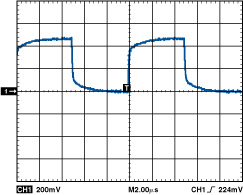
\includegraphics[width=0.3\columnwidth]{figs/probe-undercompensated}
  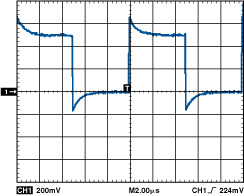
\includegraphics[width=0.3\columnwidth]{figs/probe-overcompensated}
  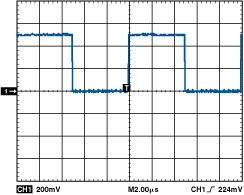
\includegraphics[width=0.3\columnwidth]{figs/probe-compensated}
  \caption{Oscilloscope probe compensation: under, over, and proper.
    From
    \url{http://www.analog.com/library/analogdialogue/archives/41-03/time_domain.html}.}
\end{figure}


\subsection{Normal mode}
\label{normal-mode}

This mode is for measuring transient or non-repetitive signals, such a
serial bus waveforms. It will only refresh the display if a trigger
event is detected.  You need to adjust the trigger level.

It is useful to increase the trigger holdoff to prevent triggering on
multiple edges of a waveform.  By default, it is set to a ridiculously
small value.

\subsection{Auto mode}
\label{auto-mode}

This mode is for measuring AC or DC signals. It is like normal mode
but if it does not detect a trigger it will automatically refresh the
display.

\section{SAM4S not detected by OpenOCD}
\label{sam4s-not-detected-by-openocd}

OpenOCD communicates with the SAM4S using either JTAG or SWD serial
interfaces.  The following assumes SWD as used by the ST-link
programmer.  SWD is a two wire bus with a clock signal and a
bi-directional data signal.


\subsection{SAM4S never detected by OpenOCD}

If the SAM4S has been previously programmed, say it has been removed
from a previous project, \hyperref[erasing-flash-memory]{erase flash
  memory} and try reconnecting with OpenOCD.

%
\begin{enumerate}
\item
  Check orientation of the SAM4S (the small circle marks pin 1).

\item
  Check 3.3\,V and 1.2\,V power rails; none of them are optional.  The
  ST-link programmer should provide 3.3\,V and the internal regulator
  in the SAM4S provides 1.2\,V.

\item
  Check the serial wire debug (SWD) signals, see
  \protect\hyperref[debugging]{debugging serial wire debug (SWD)}.
  Note, there are two variations of the ST-link programmer.

\item
  Check soldering of the SAM4S pins under a microscope.  Giving
  each pin a push with a sharp spike can reveal a poorly soldered joint.

\end{enumerate}


\subsection{SAM4S stops being detected by OpenOCD}

If OpenOCD stops working after a program is loaded,
\protect\hyperref[checking-the-crystal-oscillator]{check the crystal
  oscillator}.  This is because the crystal oscillator is selected for
the SAM4S clock when a program starts to run.  Before the SAM4S is
programmed, it uses an internal RC oscillator.

If this does not work, \hyperref[erasing-flash-memory]{erase flash
  memory} and reprogram the SAM4S with a LED flash program.  If this
works, you may have something wrong with your program.


\subsection{Erasing flash memory}
\label{erasing-flash-memory}

\begin{enumerate}
\item Connect the ERASE pin to 3.3\,V.

\item Re-start OpenOCD.

\item Re-enable \hyperref[booting-from-flash-memory]{booting from
  flash memory}.
\end{enumerate}


\subsection{Debugging serial wire debug (SWD)}
\label{debugging-serial-wire-debug-swd}

You will need a scope for this.  Hopefully you will have test-points
for the \sig{SWCK} and \sig{SWD} signals.

\begin{enumerate}
\item Check the \sig{SWCK} signal.  \program{OpenOCD} periodically
  polls to see if the SAM4S is alive.  These occur every 100\,ms, see
  \reffig{openocd-poll}.  OpenOCD polls less often when it does not
  get a response. The period increases to 6.3\,s.

\item Zoom in on the \sig{SWCK} signal.  Each spike should look like a
  clock signal.  If it is not periodic, you may have the \sig{SWD} and
  \sig{SWCK} signals transposed\footnote{There are two versions of the
    ST-link programmer.  They look identical!}.

\item Cehck the \sig{SWD} signal.  If the SAM4S responds, the waveform
  seen in \reffig{openocd-response} should be observed on the
  \sig{SWD} pin.  Note, you will need to zoom in on the waveform.
\end{enumerate}


\begin{figure}[!h]
\centering
\includegraphics[height=2.60417in]{figs/OpenOCDTimingGood.png}
\caption{OpenOCD polls every 100\,ms while connected.  Note, zooming
  in on the spikes reveals serial data packets.}
\label{fig:openocd-poll}
\end{figure}

\begin{figure}[!h]
\centering
\includegraphics[height=2.60417in]{figs/OpenOCDPollingGood.png}
\caption{\sig{SWD} signal when there is a response from the SAM4S.
  The decaying waveform at the end occurs when the pin is tri-stated.}
\label{fig:openocd-response}
\end{figure}


The common problems are:
%
\begin{itemize}
\item No power for SAM4S, 3.3\,V and 1.2\,V.  The 3.3\,V should be
  supplied by the ST-link programmer and the SAM4S internal regulator
  produces 1.2\,V.

\item The \sig{SWD} and \sig{SCK} signals are transposed.  Note, there
  are two variants of the ST-link programmer with different pin-outs!

\item The \sig{SWD} and \sig{SCK} pins are not correctly soldered.
  Check these signals with a scope on the pins of the SAM4S.

\item The SAM4S has been programmed to use the crystal oscillator but
  it is not running, see
  \protect\hyperref[checking-the-crystal-oscillator]{checking the
    crystal oscillator}.
\end{itemize}



\subsection{Checking the crystal oscillator}
\label{checking-the-crystal-oscillator}

When the SAM4S is first powered up it uses an internal RC oscillator.
However, when a program is loaded, the code before main is called
switches the SAM4S to use the main oscillator that uses the external
crystal.  If there is a problem with the crystal oscillator the SAM4S
will not run since it has no clock.  Moreover, \program{OpenOCD} will
then fail to communicate with the SAM4S.

\begin{figure}[!h]
\centering
\includegraphics[height=2.60417in]{figs/ClockSignal.png}
\caption{12\,MHz clock sine wave measured on the XOUT pin.}
\label{fig:xout}
\end{figure}

\begin{figure}[!h]
  \centering
  \mtodo{Add scope picture of CPU clock signals when not working}
  \caption{Oscillator waveform when not working.}
\end{figure}

\begin{enumerate}
\item Connect a scope pin to the \sig{XOUT} pin. A 12\,MHz sinewave
  should be visible, see \reffig{xout}.

\item If there is no sinewave:

  \begin{enumerate}
  \item Measure the voltage on the \sig{VDDPLL} pin of the MCU with a
    scope. This should be 1.2\,V to power the oscillator.

  \item Check the bypass capacitors across the crystal.  These should
    be approx. 20 pF.

  \item Check the \sig{XIN} and \sig{XOUT} solder connections under a
    microscope.
  \end{enumerate}
\end{enumerate}


\subsection{Checking the CPU clock}
\label{checking-the-clock}

The SAM4s has multiple clock sources:

\begin{enumerate}
\item
  Internal fast RC oscillator (this is selected when the SAM4S is first
  ever used).
\item
  Internal slow RC oscillator (this can be selected to save power).
\item
  Main oscillator using external crystal (this is selected when you
  run a program).
\end{enumerate}

The SAM4S uses a phase-locked-loop (PLL) to multiply the frequency of
the clock source to provide the CPU clock.  When a program is loaded,
the SAM4S is configured so that the 12\,MHz crystal oscillator
frequency is multiplied by 16 to 192\,MHz by the PLL and then divided
by 2 to provide the 96\,MHz CPU clock\footnote{The CPU can run at
  speeds up to 120\,MHz by choosing \code{MCU_PLL_MUL} and
  \code{MCU_PLL_DIV} in \file{target.h}.  The USB peripheral needs to
  run at 48\,MHz so either the CPU clock needs to be a multiple of
  48\,MHz or the second PLL needs to be configured for the USB
  peripheral.}.

\begin{enumerate}
\item Sometimes the PLL will run without a clock source and thus will
  generate an unexpected frequency.  The clock frequency can be
  checked by connecting a scope to a peripheral pin that generates a
  clock, e.g., PWM, SCK, TXD, and programming the peripheral.

  Alternatively, the PLL frequency can be checked using the OpenOCD
  \code{at91sam4s info} command, see
  \hyperref[communicating-with-openocd-using-telnet]{communicating
      with OpenOCD using telnet}.

\item The PLL requires a well regulated power supply.  Check that the
  100\,nF capacitor is not too far from the \sig{VDDPLL} pin.
\end{enumerate}


\section{LED testing}
\label{debugging-LED}

The most common reason why an LED does not work is that you have
incorrectly specified its PIO pin in the \file{target.h} file (see
\protect\hyperref[configuration]{configuration}).

An active-high LED should faintly glow before the SAM4S is first
programmed.  This is due to the internal pullup resistors on each PIO
pin.  If the LED does not glow, check its orientation.

If the LED still does not work, use an oscilloscope to check that the
PIO pin is correctly driven.


\section{USB serial}
\label{debugging-usb}

USB is a complicated protocol and there are many possibilities why it
does not work.  First check your hardware by
\hyperref[erasing-flash-memory]{erasing flash memory} and connecting
the USB to a PC.  If a new USB device is detected, your hardware is
correct\footnote{You may have a poorly soldered connection that gives
  intermittent operation.}.  Note, you will then need to re-enable
\hyperref[booting-from-flash-memory]{booting from flash} before
loading your program.

If the hardware does not work:
%
\begin{enumerate}
  \item Check that the USB cable is not power-only, say by using a
    known good cable.

  \item
    Check that the USB termination resistors are 27\,ohms.

  \item Check the USB connector pins and the SAM4S USB pins under a
    microscope.  If they move if you push them with a sharp-pointy
    thing, resolder.

  \item
    Check that the USB signals are not transposed.

  \item Check the crystal oscillator is running at 12\,MHz, see
    \protect\hyperref[checking-the-crystal-oscillator]{checking the
      crystal oscillator}.

  \item Check that the CPU is running at 96\,MHz, see
    \protect\hyperref[checking-the-clock]{checking the CPU clock}.

  \item Try an unmodified test program in case you have introduced a
    coding error.
\end{enumerate}

If the USB serial connection drops characters:
  %
 \begin{itemize}
 \item Add a delay before sending data, e.g., \code{delay_ms (100);}.
   This is because the driver takes a while to set up the connection
   after the USB cable is plugged in.  If you try to send some data
   during this time, the data gets stored into a ring buffer for later
   transmission.  However, the ring buffer is not large and once it is
   filled, the USB serial driver will drop characters.
 \end{itemize}


\section{Motors}
\label{motors-testing}

For the motors to work:
%
\begin{enumerate}
\item The H-bridge must be correctly configured.
\item The PWM signals must be correctly generated.
\end{enumerate}


\subsection{Testing the H-bridge}
\label{testing-the-h-bridge}

\begin{enumerate}
\item The \sig{nFAULT} pin should be high.  Note, this is an
  open-drain pin and requires a pullup resistor to 3V3 to make it
  work.  Without this resistor, this pin will always read low, fault
  or no fault.  If this is connected to the SAM4S, it will be pulled
  up by default.

\item The \sig{nSLEEP} pin needs to be high to enable the chip.

\item Check that the capacitor connected to the \sig{INT} pin is
  2.2\,$\mu$F and not 2.2\,nF.

\item Check the \sig{AIN1}, \sig{AIN2}, \sig{BIN1}, \sig{BIN2} pins.
  If you see DC 2\,V, this is due to the signal not being configured
  as an output on the SAM4S; the internal pullup of the SAM4S forms a
  voltage divider with the internal pulldown of the H-bridge chip.

\item Check that \sig{AINSENSE} and \sig{BINSENSE} are connected
  directly to ground or to ground via a small resistor if you want
  current limiting.
\end{enumerate}


\subsection{Debugging PWM}
\label{debugging-pwm}

If PWM does not work:

\begin{enumerate}
\item
  Check the SAM4S pin since not every pin can be a PWM signal.  The
  SAM4S can generate four independent hardware PWM
  signals\footnote{And the complementary output.}. See
  \wfile{mat91lib/pwm/pwm.c} for a list of supported PIO pins.  Note,
  \pin{PA16}, \pin{PA30}, and \pin{PB13} are different options for
  PWM2.

\item
  Check the definition in the configuration file \file{target.h}.
\end{enumerate}

If the PWM frequency is wrong:

\begin{enumerate}
\item
  Check the clock frequency, see
  \hyperref[checking-the-clock]{checking the clock}.
\item
  Check your program.
\end{enumerate}

If the PWM duty is wrong:

\begin{enumerate}
\item
  Check your program. There are two ways to set the duty cycle with
  mat91lib's PWM module: (1) setting the \code{duty} field of the
  \code{pwm_cfg_t} struct using the \code{PWM_DUTY_DIVISOR} macro and
  passing the duty cycle as a percentage or (2) setting the
  \code{duty_ppt} field of the \code{pwm_cfg_t} struct as an integer
  in parts per thousand (e.g., 1000 = 100\% duty cycle; 50 = 5\% duty
  cycle). Setting the latter field will override the former. See the
  definition of \code{pwm_cfg_t} in \wfile{mat91lib/pwm/pwm.h}.
\end{enumerate}

\begin{figure}[!h]
\centering
\includegraphics[height=2.60417in]{figs/PWM_2.png}
\caption{Two PWM signals at 1\,kHz and 10\,kHz.}
\end{figure}


\section{IMU}
\label{imu}

For the IMU to work:
%
\begin{enumerate}
\item The IMU chip must be correctly configured.
\item The I2C bus must be working.
\end{enumerate}


\subsection{IMU checking}
\label{checking-IMU}

\begin{enumerate}
\item Check the I2C bus (see \hyperref[debugging-i2c]{debugging I2C}).
\item Check the auxiliary I2C bus signals are not connected on the IMU
  (otherwise the magnetometer will not respond).
\item Check \sig{nCS} on the IMU is pulled high.
\item Check \sig{FSYNC} on the IMU is pulled low.
\item Try pressing on a side of the IMU with a fingernail to see if it
  starts working; you might have a dry joint.  Otherwise look under
  the microscope at the pins of the IMU and touch them up with a
  soldering iron if necessary.
\item Check that you are using the correct I2C address corresponding
the the state of the AD0 pin (see datasheet).
\end{enumerate}


\subsection{Debugging I2C}
\label{debugging-i2c}

\begin{enumerate}
\item
  I2C/TWI requires external pull-up resistors for the clock (TCK) and
  data (TDA) signals.  Use a scope to look at the signals
  \pin{TWCK/SCL} and \pin{TWD/SDA}.  If the rise times are too slow so
  that the high voltage level is not 3.3\,V, the resistors are too
  large.
\item
  TWI channel 1 (TWI1) uses \pin{PB4} and \pin{PB5}. However, these
  are configured on boot as JTAG pins. You can disable this, see
  \hyperref[disabling-jtag-pins]{disabling JTAG pins}.
\end{enumerate}

The oscilloscopes in the ESL can be configured to trigger on I2C%
\footnote{They also support other serial protocols including SPI and
UART.} frames and automatically decode and display the contents of
each frame. Press the `Protocol' button on the scope then use the
touch screen to change the protocol to I2C. You will require a probe
each for the data and clock signals: touch the `Trigger' button in the
protocol menu to configure which channel corresponds to which signal.
See \reffig{i2c-ack} and \reffig{i2c-noack} for examples.

\begin{figure}[!h]
  \centering
  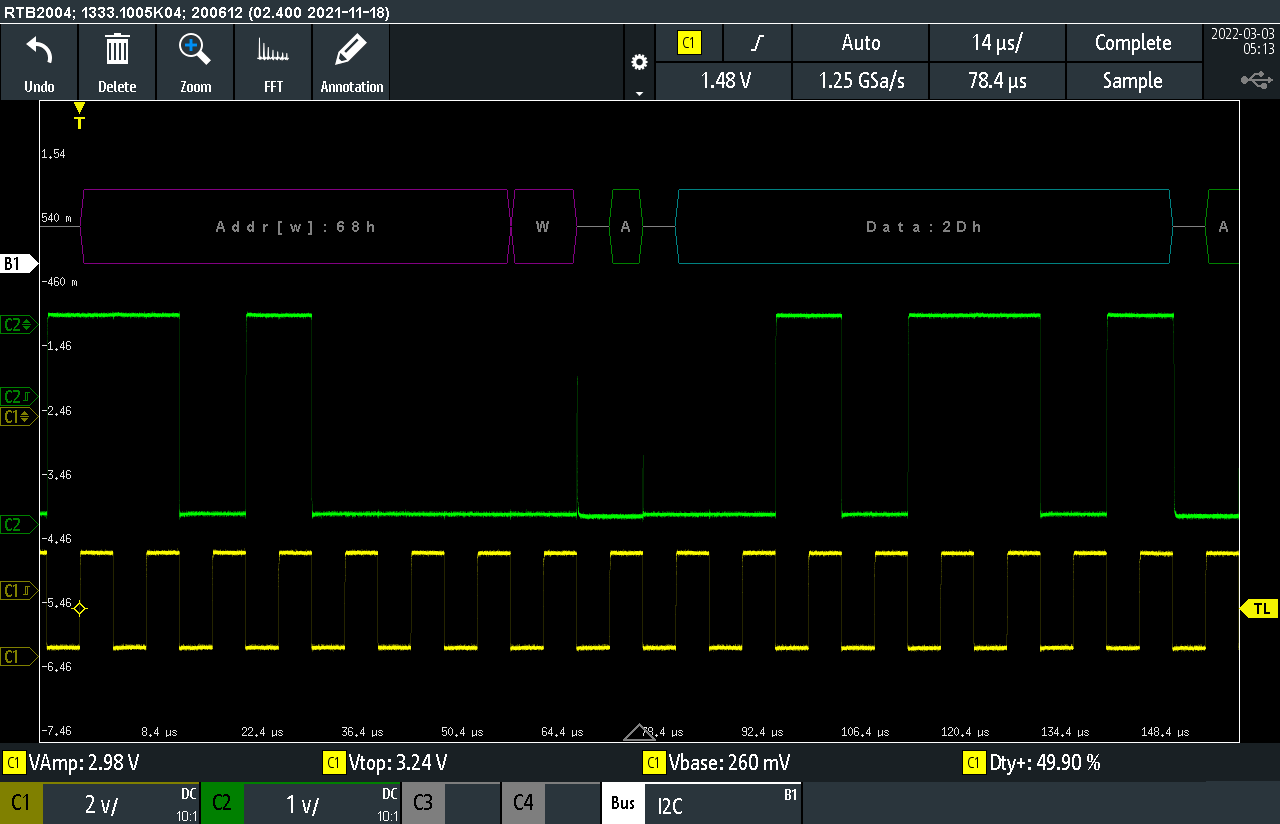
\includegraphics[width=\linewidth]{figs/i2c-ack.png}
  \caption{I2C signals with acknowledgement; the green trace is
  \code{TWD/SDA} and the yellow trace is \code{TWCK/SCL}.}
  \label{fig:i2c-ack}
\end{figure}


\begin{figure}[!h]
  \centering
  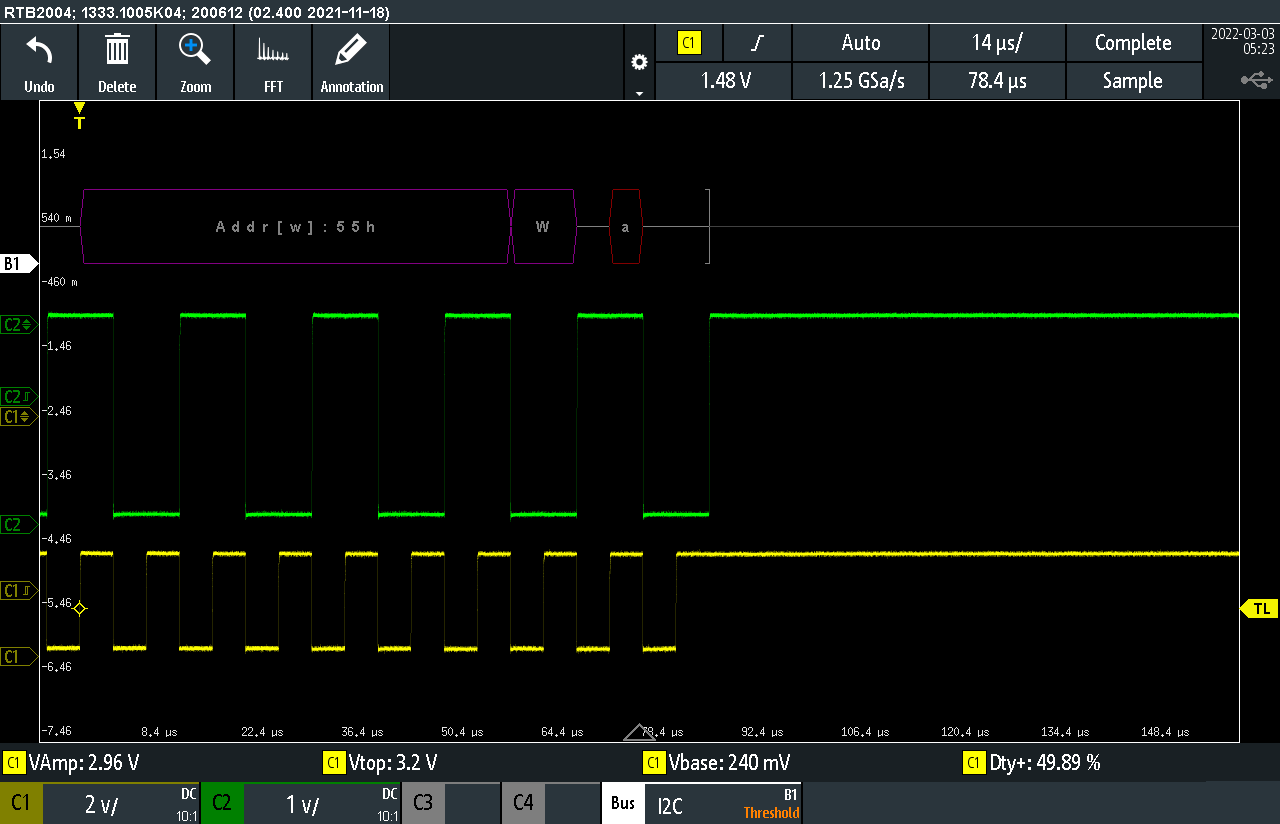
\includegraphics[width=\linewidth]{figs/i2c-noack.png}
  \caption{I2C signals with no acknowledgement; the green trace is
  \code{TWD/SDA} and the yellow trace is \code{TWCK/SCL}.}
  \label{fig:i2c-noack}
\end{figure}


\section{NRF24L01+ radio}
\label{nrf24l01-radio}

For the radio to work you need:

\begin{enumerate}
\item No ground planes near the antenna\footnote{You might have to
  mount the radio vertically.}.

\item A working SPI interface.

\item The correct channel and address.

\item A well filtered power supply for the radio, see \reffig{radio-filtering}.

\item A channel with little interference (note, some channels are
  shared with WiFi and Bluetooth and may be less reliable).
\end{enumerate}

If nothing works, check:

\begin{enumerate}
\item
  For transmission the CE pin should be low; for reception the CE pin
  should be high.
\item
  Check that the SPI clock SCK, MOSI, and MISO signals are driven when
  the radio is configured (note, the MISO signal is tristate when CS is
  high).
\item
  Check that the SPI CS signal is driven low for each transmitted byte.
\end{enumerate}

If the radio transmits but not receives, check:

\begin{enumerate}
\item
  The IRQ pin is driven low (this indicates that a packet has been
  received).
\item
  The power supply. The radio requires a well filtered power supply
  otherwise the range will be limited on reception. Preferably, the
  device should have its own 3V3 regulator with a low-pass RC filter
  comprised of a series resistor and large capacitor (say 22\,$\mu$F)
  or a low-pass LC filter made with a ferrite bead and capacitor.
\end{enumerate}

\textbf{Note}, by default the radio waits for an auto-acknowledgement
from the receiver device. This acknowledgement is performed in hardware.
If no acknowledgement is received, it retries for up to 15 times. The
auto-acknowledgement and number of retries can be configured in
software.

\subsection{Checking the radio power supply}
\label{checking-the-radio-power-supply}

\begin{figure}[!h]
  \centering
  \mtodo{Add scope picture of expected radio power supply voltage}
  \caption{Waveform showing radio power supply voltage.}
\end{figure}


\subsection{Debugging SPI}
\label{debugging-spi}

Check:
%
\begin{enumerate}
\item The device chip select signal is driven low.
\item The \pin{SCK} signal toggles while the chip select is low.
\item The \pin{MOSI} signal does something while the chip select is low.
\end{enumerate}
%
The \pin{MISO} signal is usually tri-state and is driven by the
device when the chip select is low.

The SPI standard is rather loose and there are four modes to confuse
the unwary; these are due to two clock polarity modes and two clock
phase modes.  When using the wrong mode, the read data can be out by a
bit or unreliable.

\begin{figure}[!h]
  \centering
  \mtodo{Add scope picture of SPI signals}
  \caption{SPI signals.}
\end{figure}


\subsection{Debugging ADC}
\label{debugging-adc}

If the ADC does not work:
%
\begin{enumerate}
\item
  Check the SAM4S pin since not every pin can be an ADC input.

\item
  Check the definition in the configuration file \file{target.h}.

\item
  Check that the SAM4S \sig{VDDVREF} pin is 3.3\,V.

\end{enumerate}


\subsection{Debugging the LED tape}

If the LED tape does not work:
%
\begin{enumerate}
\item Check that it is supplied with 5\,V.

\item Check that there is a data signal with 5\,V logic (the level
  translator may be configured for the wrong direction).

\item Change the timing parameter in the LED tape driver.  It appears
  that some LED tapes have different timing specifications.
\end{enumerate}



\section{Other problems}
\label{faq}

\begin{enumerate}
\item
  \emph{\program{OpenOCD} does not run}. The most common problem is
  that the USB permissions are not correct\footnote{On Linux this is
    controlled by udev.}.

\item
  \emph{A program does not correctly build after a file has been
    changed}. Every now and then the file timestamps are incorrect
  (this is a common problem with network drives due to a skew in the
  clocks) and make will not correctly rebuild a file. Running
  \textbf{make clean} will remove the existing dependency and object
  files so you can start afresh.

\item
  \emph{A program hangs.} This can be observed by an LED no longer
  flashing. There are a number of reasons:

  \begin{enumerate}
  \item
    The program is stuck in an infinite loop. Note, an embedded system
    should only have an infinite loop for the main loop; all other loops
    should have a timeout condition.
  \item
    The program has crashed trying to access invalid memory. Usually
    this is due to buffer overflow or dereferencing uninitialised
    pointers (say by not calling \code{radio_init}). Try running
    \code{make debug}.  This will start the
    \protect\hyperref[debugging]{debugger} and attach to your MCU. If
    the debugger says that your program has stopped in
    \code{_hardfault_handler}, then your program is likely to have
    accessed invalid memory. Use the \code{bt} command to print a
    stack trace to see how your program went astray.

  \item You are printing output using USB but a terminal program is
    not running.
  \end{enumerate}

\item
  \emph{The output of the 3V3 regulator works fine when powered from
    USB but gives 6\,V when powered from a 7.2\,V battery}. Check that
  the 7.2\,V is not connected directly to a SAM4S pin (say for battery
  monitoring) since this will cause an ESD protection diode inside the
  SAM4S to conduct.

\item \emph{Sometimes the program works but other times it does not}
  The likely causes are:
  %
  \begin{enumerate}
  \item You have an uninitialised variable---check your code.

  \item You have a poor solder connection for a MCU pin---check with
    microscope.

  \item You have a race condition---this is unlikely unless you are
    using interrupts.

  \item Your power supply might be slow to rise up to operating
    voltage.  Try adding a delay, for example, \code{delay_ms (100);},
    at the start of \code{main}.
  \end{enumerate}

\item \emph{The SAM4s works but randomly dies} The likely cause is
  having the decoupling capacitors too far away ($> 2$\,cm).

\end{enumerate}

\chapter{Rework}


\section{Removing resistors and capacitors}

\begin{enumerate}
\item Apply flux from syringe to pads.

\item Use tweezer soldering iron.
\end{enumerate}


\section{Removing larger parts}


\begin{enumerate}
\item Apply flux from syringe to pads.

\item Use a grunty soldering iron.  \textbf{Do not push hard with a
  small soldering iron since this will bend the tips.}
\end{enumerate}



\section{Removing MCU}

\begin{enumerate}
\item Apply flux from syringe to all pins.

\item Get Scott to show you how to use the hot-air gun.  They key is
  to choose a head that matches the size of the MCU.
  
\end{enumerate}



\section{Adding a wire}

\begin{enumerate}
\item For a signal trace, choose the very fine wire.

\item Cut to length and strip insulation from both ends.  The second
  end is a lot harder!

\item Bend wire to shape and tape down to the PCB.  Note, you can run
  this wire through vias.

\item Apply flux from syringe to both pads.

\item Use small soldering iron.  
\end{enumerate}

\chapter{Debugging}
\label{debugging}

Your SAM4S can be debugged using \hyperref[OpenOCD]{OpenOCD} in
conjunction with GDB.  However, debugging embedded systems is
difficult due to asynchronous behaviour.  Moreover, when optimising, a
compiler will rearrange (and even remove) code and hold variables in
registers.

\section{Command-line debugging with GDB}

If \program{OpenOCD} is running, a running program can be debugged using:

\begin{minted}{bash}
$ make debug
\end{minted}

This starts \program{GDB} and attaches to the SAM4S. \program{GDB} is
a command line debugger but there are many GUI programs that will
control it, for example, \program{vscode} and \program{geany} have
plugins.

\program{GDB} allows you to inspect the CPU registers, memory, set
breakpoints, set watchpoints, and much more.

You can reset your program using the GDB \code{jump reset} command.
However, this does not reset the peripherals as with a power-on reset.

The backtrace, \code{bt}, command is useful to show the function call
stack.





\appendix
\chapter{OpenOCD}
\label{OpenOCD}

The Open On-Chip Debugger (OpenOCD) is an open-source on-chip
debugging, in-system programming, and boundary-scan testing tool. It
is able to communicate with various ARM and MIPS microprocessors via
\wikiref{JTAG}{JTAG} or \wikiref{SWD}{SWD}. It works with a number of
different \wikiref{JTAG}{JTAG} or \wikiref{SWD}{SWD}
interfaces/programmers. User interaction can be achieved via
\file{telnet/putty} or the GNU debugger (GDB).


\section{Configuration files}
\label{configuration-files}

OpenOCD needs a \wikiref{OpenOCD_configuration}{configuration file} to
specify the interface (USB or parallel port) and the target system.
Unfortunately, these change with every new release of OpenOCD.


\section{Running OpenOCD}
\label{running-openocd}

OpenOCD runs as a daemon program in the background and can be
controlled from other programs using TCP/IP sockets. This means that
you can remotely debug from another computer. The socket ports it uses
are specified in the \wikiref{OpenOCD_configuration}{OpenOCD
  configuration} file supplied when it starts. By default, OpenOCD
uses port 3333 for \wikiref{GDB}{GDB} and port 4444 for general
interaction using the \file{telnet} program.


\subsection{Communicating with OpenOCD using telnet}
\label{communicating-with-openocd-using-telnet}

If OpenOCD is running, commands can be sent to it using the telnet
program.  For example,
%
\begin{minted}{bash}
$ telnet localhost:4444
> halt
> at91sam4 info
\end{minted}
%
To exit use \code{ctrl-]} then \code{c}.  On Windows, you can use the
  \file{putty} program.


\subsection{Communicating with OpenOCD using GDB}
\label{communicating-with-openocd-using-gdb}

If OpenOCD is running, commands can be set to it with
\wikiref{GDB}{GDB}. There are two steps: connecting to OpenOCD with
the target remote command, and then sending a command with the GDB
monitor command. For example,

\begin{minted}{bash}
$ gdb
(gdb) target remote localhost:3333
(gdb) monitor flash info 0
\end{minted}

\section{OpenOCD commands}
\label{openocd-commands}

All the gory OpenOCD details can be found in the
\wikiref{Media:openocd.pdf}{OpenOCD manual}. If you are getting strange
errors see \wikiref{OpenOCD_errors}{OpenOCD errors}.

\section{Flash programming}
\label{flash-programming}

OpenOCD can program the flash program memory from a binary file.

%% \section{FTDI support}
%% \label{ftdi-support}

%% Many \wikiref{JTAG_interface}{JTAG interfaces} use chips made by Future
%% Technology Devices International (FTDI) to translate between the USB and
%% JTAG protocols. FTDI provide a library to communicate with these
%% devices; however, this is not open-source and hence cannot be
%% distributed. There is an open-source equivalent,
%% \href{http://freshmeat.net/projects/libftdi/}{libftdi}, which in turn
%% uses the open-source libusb. This can be temperamental to get working on
%% a Windows system.

%% \section{Getting OpenOCD}
%% \label{getting-openocd}

%% The developers of OpenOCD release source packages (and provide
%% subversion access) but do not provide official builds for any
%% operating system. However, there are various sites which provide
%% pre-built versions of OpenOCD.

%% \subsection{Windows}
%% \label{windows}

%% Windows installers for release versions of OpenOCD can be found
%% \href{http://www.freddiechopin.info/index.php/en/download/category/4-openocd}{here}.
%% Some development versions can be found
%% \href{http://www.freddiechopin.info/index.php/en/download/category/10-openocd-dev}{here}.
%% Unless you need a feature not present in the release version, avoid
%% getting the development versions as they can be less stable.

%% Alternatively, the
%% \href{http://www.siwawi.arubi.uni-kl.de/avr_projects/arm_projects/}{WinARM}
%% toolchain contains a version of OpenOCD, albeit one that appears (from
%% the description on the project page) to be out of date. It is also
%% possible to build your own copy of OpenOCD using either
%% \href{http://www.mingw.org/}{MinGW} or
%% \href{http://www.cygwin.com/}{Cygwin}; instructions for this are posted
%% in various places online.

%% Realistically, it's probably easier to set up a virtual machine with
%% Linux and use that instead.

%% \subsection{Linux}
%% \label{linux}

%% Many recent distributions of Linux have OpenOCD in their software
%% repositories. However, this is often out of date and (in some cases)
%% buggy. In this case it is straightforward to
%% \wikiref{Building_OpenOCD_under_Linux}{build the latest version}.

%% \subsection{Mac OSX}
%% \label{mac-osx}

%% The easiest way to install OpenOCD on Mac OSX is to use
%% \href{http://brew.sh/}{Homebrew}. If you wish to use JTAG with an
%% adaptor based on a FTDI chip (for example, the UCECE USB to JTAG
%% adaptor or a Bus Blaster), make sure you include libftdi support by
%% installing with the command:
%% %
%% \begin{minted}{bash}
%% $ brew install openocd --enable-ft2232_libftdi
%% \end{minted}

\section{System information}
\label{system-information}


The openocd command \code{at91sam4 info}, see
\hyperref[communicating-with-openocd-using-telnet]{communicating with
  OpenOCD using telnet}, outputs useful information about the state of
the SAM4S.  For example:
%
\begin{verbatim}
    CKGR_MOR: [0x400e0420] -> 0x01006409
	    MOSCXTEN:     1 [0x0001] (main xtal enabled: YES)
	    MOSCXTBY:     0 [0x0000] (main osc bypass: NO)
	    MOSCRCEN:     1 [0x0001] (onchip RC-OSC enabled: YES)
	     MOSCRCF:     0 [0x0000] (onchip RC-OSC freq: 4 MHz)
	    MOSCXTST:   100 [0x0064] (startup clks, time= 3051.757812 uSecs)
	     MOSCSEL:     1 [0x0001] (mainosc source: external xtal)
	       CFDEN:     0 [0x0000] (clock failure enabled: NO)
   CKGR_MCFR: [0x400e0424] -> 0x000117ac
	    MAINFRDY:     1 [0x0001] (main ready: YES)
	       MAINF:  6060 [0x17ac] (12.411 Mhz (32.768khz slowclk)
  CKGR_PLLAR: [0x400e0428] -> 0x08133f01
	        DIVA:     1 [0x0001]
	        MULA:    19 [0x0013]
	PLLA Freq: 248.218 MHz
   CKGR_UCKR: [0x400e041c] -> 0x00000000
    PMC_FSMR: [0x400e0470] -> 0x00000000
    PMC_FSPR: [0x400e0474] -> 0x00000000
     PMC_IMR: [0x400e046c] -> 0x00000000
    PMC_MCKR: [0x400e0430] -> 0x00000012
	         CSS:     2 [0x0002] plla (248.218 Mhz)
	        PRES:     1 [0x0001] (clock/2)
		Result CPU Freq: 124.109
    PMC_PCK0: [0x400e0440] -> 0x00000000
    PMC_PCK1: [0x400e0444] -> 0x00000000
    PMC_PCK2: [0x400e0448] -> 0x00000000
    PMC_PCSR: [0x400e0418] -> 0x41004000
    PMC_SCSR: [0x400e0408] -> 0x00000001
      PMC_SR: [0x400e0468] -> 0x0003000f
 CHIPID_CIDR: [0x400e0740] -> 0x289c0ae0
	     Version:     0 [0x0000]
	       EPROC:     7 [0x0007] Cortex-M4
	     NVPSIZE:    10 [0x000a] 512K bytes
	    NVPSIZE2:     0 [0x0000] none
	    SRAMSIZE:    12 [0x000c] 128K Bytes
	        ARCH:   137 [0x0089] ATSAM3S/SAM4S xB Series (64-pin version)
	      NVPTYP:     2 [0x0002] embedded flash memory
	       EXTID:     0 [0x0000] (exists: NO)
 CHIPID_EXID: [0x400e0744] -> 0x00000000
   rc-osc: 4.000 MHz
  mainosc: 12.411 MHz
     plla: 248.218 MHz
 cpu-freq: 124.109 MHz
mclk-freq: 124.109 MHz
 UniqueId: 0x53343100 0x50524a46 0x36303430 0x30363030
\end{verbatim}
%
Note, the reported clock frequencies are not accurate.


\section{Errors}
\label{openocd_errors}

\verb+Error: libusb_open() failed with LIBUSB_ERROR_ACCESS+ On Linux
you need to give permissions to access the USB.  You can do this by
finding the file \file{99-openocd.rules} that comes with the OpenOCD
distribution and then:
%
\begin{minted}{bash}
  $ sudo cp 99-openocd.rules /etc/udev/udev.rules
  $ sudo udevadm control --reload
\end{minted}
%
Finally, you need to reconnect the ST-link device.


See also \wikiref{OpenOCD_errors}{OpenOCD errors}.


\section{Programming without GDB}

OpenOCD can program the SAM4S without using GDB.  You will need to
kill any currently running instance of OpenOCD and then use:
%
\begin{minted}{bash}
  $ openocd -f path-to-sam4s-stlink.cfg -c "program program.bin verify reset exit"
\end{minted}
%
Here \file{program.bin} is the name of the program to load.

\chapter{Git}
\label{git}

To properly use git you should commit and push often. The smaller the
changes and the more often you make per commit, the smaller the chance
of the dreaded merge conflict.


\section{Typical workflow}

\begin{enumerate}
\item Edit file

\item Save changes

\item Check differences

\begin{minted}{bash}
    $ git diff .
\end{minted}

\item Commit changes

\begin{minted}{bash}
    $ git commit -m "Commit message" list-of-modified-files
\end{minted}

Note, you should commit at least every 15 min, preferably when you
have made a single functional change.  Ideally each commit should be
self-contained.  \textbf{Note, do not add binary files (.o) etc.}
These will make merging even more miserable.

\item Push changes to server

\begin{minted}{bash}
    $ git push
\end{minted}

The more often you push, the lower the chance that you will get a
merge conflict.

\end{enumerate}


\section{Diff, status, blame, log}

The diff command is useful to determine what changes you made.

The status command says which files have been modified and what you
should do, say when you get a merge conflict.

The blame command is useful to determine who authored each line of code.

The log command shows all the previous commit messages.


\section{Pulling from upstream}
\label{git-pulling-from-upstream}

To be able to get updates if the template project is modified you will
need to:

\begin{minted}{bash}
$ cd wacky-racers
$ git remote add upstream https://eng-git.canterbury.ac.nz/wacky-racers/wacky-racers-2021.git
\end{minted}

Again if you do not want to manually enter your password (and have
ssh-keys uploaded) you can use:
%
\begin{minted}[breaklines]{bash}
$ cd wacky-racers
$ git remote add upstream git@eng-git.canterbury.ac.nz:wacky-racers/wacky-racers-2021.git
\end{minted}

Once you have defined the upstream source, to get the updates from the
main repository use:
%
\begin{minted}{bash}
$ git pull upstream master
\end{minted}

If you enter the wrong URL by mistake, you can list the remote servers
and delete the dodgy entry:

\begin{minted}{bash}
$ git remote -v
$ git remote rm upstream
\end{minted}

Note, \textbf{origin} refers to your group project and \textbf{upstream}
refers to the template project that origin was forked from.

\section{Merging}
\label{git-merging}

The bane of all version control programs is dealing with a merge
conflict. You can reduce the chance of this happening by committing and
pushing faster than other people in your group.

If you get a message such as:
%
\begin{verbatim}
From https://eng-git.canterbury.ac.nz/wacky-racers/wacky-racers-2021
 * branch            master     -> FETCH_HEAD
error: Your local changes to the following files would be overwritten by merge:
    src/test-apps/imu_test1/imu_test1.c
Please, commit your changes or stash them before you can merge.
\end{verbatim}
%
what you should do is:
%
\begin{minted}{bash}
$ git stash
$ git pull
$ git stash pop
# You may now have a merge error and will have to edit the problem file, in this case imu_test1.c
# Once the file has been fixed
$ git add src/test-apps/imu_test1/imu_test1.c
$ git commit -m "Fix merge"
\end{minted}

Sometimes when you do a git pull you will be thrown into a text editor
to type a merge comment. The choice of editor is controlled by an
environment variable \code{EDITOR}. On the ECE computers this defaults
to emacs\footnote{To exit emacs type ctrl-x ctrl-c, to exit vi or vim
  type \code{:q!}.}  on Linux. You can changed this by adding a line
such as the following to the \file{.bash\_profile} file in your home
directory.

\begin{minted}{bash}
$ export EDITOR=geany
\end{minted}

\chapter{Sleeping}

Sleeping a MCU is important for embedded systems applications to
prolong battery life.


\section{Dynamic power consumption}

The dynamic power consumption for CMOS is
%
\begin{equation}
  P = f C V^2,
  \label{eqn:power}
\end{equation}
%
where $f$ is the clock frequency, $C$ is the total switched
capacitance, and $V$ is the power supply voltage.  It can be difficult
to reduce $V$ for a MCU and so the power consumption can only be
reduced by lowering the clock frequency, $f$, and/or shutting down
parts of the MCU to reduce $C$.


\section{Slowing the CPU clock}

The SAM4S, like many MCUs, can be clocked from a number of sources.
For example, it has a slow clock generated by an RC oscillator with a
frequency of 32768\,Hz.

With the mat91lib library the slow clock can be selected using:
%
\begin{minted}{C}
    mcu_select_slowclock ();
\end{minted}

\textbf{Warning}, switching to a slow CPU clock will cause havoc with
OpenOCD.  You might not be able to load a new program.  In this case,
you will need to \hyperref[erasing-flash-memory]{erase flash memory}.


\section{Disabling the CPU clock}

Further power reduction can be achieved by disabling the CPU clock.
In effect, this reduces $C$ in \refeqn{power}.  The clock is disabled
using the ARM WFI (wait for interrupt) instruction.  The clock remains
disabled until an interrupt occurs.  The WFI instruction is executed
by calling the mat91lib \code{cpu_wifi ()} function, defined as:
%
\begin{minted}{C}
static inline void
cpu_wfi (void)
{
    __asm__ ("\twfi");
}
\end{minted}

\textbf{Warning}, before executing the WFI instruction, it is necessary
to enable an interrupt to wake the CPU.

\textbf{Warning}, disabling the CPU clock will cause havoc with
OpenOCD.


\section{Disabling peripherals}

Further power reduction can be achieved by shutting down peripherals
that are not required.  This also reduces $C$ in \refeqn{power}.  The
drivers in mat91lib have a shutdown function, e.g., \code{spi_shutdown
  ()}.



\section{Current measurement}

Measuring the current to determine power consumption is not
straightforward.  Usually, the voltage drop across a known resistance
is measured.  For normal operation, this resistance needs a low value
otherwise there will be significant voltage drop and the MCU will not
run.  When sleeping, a much larger resistor is required so that the
voltage drop can be measured (all going well the MCU will only take a
few microamps when sleeping).  One approach is to use two voltage drop
resistors connected in parallel when the MCU is running normally, and
to switch out the low value one when the MCU is sleeping.  There are
special current measuring devices that dynamically vary the voltage
drop resistor.





\chapter{EMC}


Electromagnetic emission (EMI) occurs with changing electric and
magnetic fields.  A good PCB design should have good electromagnetic
compatibility (EMC); this means that it has low EMI and that is has
low susceptibility to changing electric and magnetic fields.


\section{Electromagnetic coupling}

It is worth recapping the fundamental equations.  A changing aggressor
current, $i_a(t)$, flowing around a loop induces a
voltage\footnote{This voltage magically appears around a loop and does
  not obey Kirchhoff's voltage law.  It will mostly `appear' across
  the highest resistance in the loop.} in a victim loop according to
Faraday's law,
%
\begin{equation}
  v_v(t) = M \frac{\ud i_a(t)}{\ud t},
\end{equation}
%
where $M$ is the mutual inductance.  The mutual inductance depends on
the areas of the aggressor and victim loops and their orientation.

A changing aggressor voltage induces a current in a victim circuit
according to
%
\begin{equation}
  i_v(t) = C \frac{\ud v_a(t)}{\ud t},
\end{equation}
%
where $C$ is the mutual capacitance.  From Ohm's law, this will
produce a voltage $i_v(t) R$ across a resistance $R$.

\chapter{PIO pins}


%\section{PIO output resistance}

There are five types of PIO driver, see \reftab{pio-pins}, with
different drive strengths.  The SPI signals are designed for 70\,MHz
operation and require greater drive strengths.  Each
pin\footnote{Except the USB pins; these need external 27\,ohm series
  termination resistors.} has a series resistor for on-die-termination
(ODT) to reduce reflections.  The maximum current applies for DC
operation; the drivers can momentarily provide much more current.



\begin{table}
  \begin{tabular}{lllllll}
    Pin     & Pin group & ODT & Imax (mA) & fmax (MHz) & Speciality    \\ \hline    
    PA0     &  4 & 18 &  2 & 58 &       \\
    PA1     &  4 & 18 &  2 & 58 &       \\
    PA2     &  4 & 18 &  2 & 58 &       \\
    PA3     &  4 & 18 &  2 & 58 & TWD0  (TWI)      \\
    PA4     &  2 & 36 &  2 & 46 & TWCK0 (TWI)      \\
    PA5     &  2 & 36 &  2 & 46 &       \\
    PA6     &  2 & 36 &  2 & 46 &       \\
    PA7     &  2 & 36 &  2 & 46 &       \\
    PA8     &  2 & 36 &  2 & 46 &       \\
    PA9     &  2 & 36 &  2 & 46 &       \\
    PA10    &  2 & 36 &  2 & 46 &       \\
    PA11    &  2 & 36 &  2 & 46 &       \\
    PA12    &  3 & 36 &  2 & 70 & MISO (SPI)      \\
    PA13    &  3 & 36 &  2 & 70 & MOSI (SPI)      \\
    PA14    &  1 & 36 &  4 & 70 & SPCK (SPI)      \\
    PA15    &  2 & 36 &  2 & 46 & TF (SSC)      \\
    PA16    &  2 & 36 &  2 & 46 & TK (SSC)      \\
    PA17    &  2 & 36 &  2 & 46 & TD (SSC)      \\
    PA18    &  2 & 36 &  2 & 46 & RD (SSC)      \\
    PA19    &  2 & 36 &  2 & 46 & RK (SSC)      \\
    PA20    &  2 & 36 &  2 & 46 & RF (SSC)      \\
    PA21    &  2 & 36 &  2 & 46 &       \\
    PA22    &  2 & 36 &  2 & 46 &       \\
    PA23    &  2 & 36 &  2 & 46 &       \\
    PA24    &  2 & 36 &  2 & 46 &       \\
    PA25    &  2 & 36 &  2 & 46 &       \\
    PA26    &  3 & 36 &  2 & 70 & MCDA2 (multimedia)      \\
    PA27    &  3 & 36 &  2 & 70 & MCDA3 (multimedia)      \\
    PA28    &  3 & 36 &  2 & 70 & MCCDA (multimedia)      \\
    PA29    &  1 & 36 &  4 & 70 & MCCK (multimedia)       \\
    PA30    &  3 & 36 &  2 & 70 & MCDA0 (multimedia)      \\
    PA31    &  3 & 36 &  2 & 70 & MCDA1 (multimedia)      \\
    PB0     &  2 & 36 &  2 & 46 &       \\
    PB1     &  2 & 36 &  2 & 46 &       \\
    PB2     &  2 & 36 &  2 & 46 &       \\
    PB3     &  2 & 36 &  2 & 46 &       \\
    PB4     &  2 & 36 &  2 & 46 & TDI (JTAG)      \\
    PB5     &  2 & 36 &  2 & 46 & TDO (JTAG)     \\
    PB6     &  2 & 36 &  2 & 46 & TMS (JTAG)     \\
    PB7     &  2 & 36 &  2 & 46 & TCK (JTAG)     \\
    PB8     &  2 & 36 &  2 & 46 & XOUT (crystal)    \\
    PB9     &  2 & 36 &  2 & 46 & XIN  (crystal)    \\
    PB10    &  5 & 0  & 30 & 25 & DDM (USB)       \\
    PB11    &  5 & 0  & 30 & 25 & DDP (USB)      \\
    PB12    &  2 & 36 &  2 & 46 & ERASE      \\
    PB13    &  2 & 36 &  2 & 46 & DAC0      \\
    PB14    &  2 & 36 &  2 & 46 & DAC1      \\
  \end{tabular}
  \caption{SAM4S PIO pins.}
  \label{tab:pio-pins}
\end{table}

%\chapter{Assessment}




\end{document}
